\section{The steady state}
%
The steady state is achieved as described in \cref{sec:initRun}.
We will in this section discuss the resulting profiles.

\subsection{Parallel profiles}

FIXME: Consider to remove ln(n), vortD, nui from the profiles.

%
\begin{figure}[htb]
    \centering
    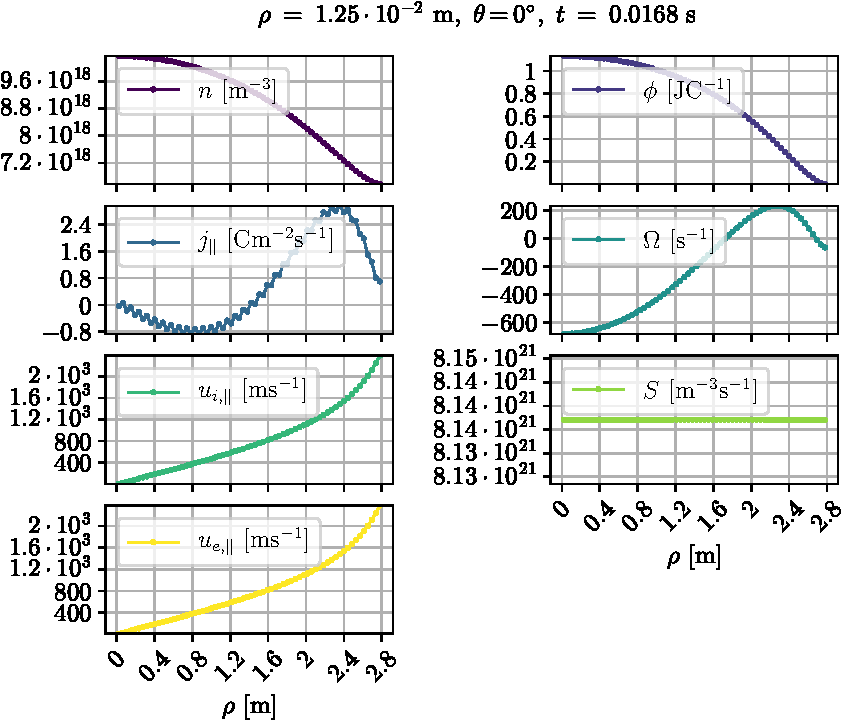
\includegraphics[width=1.0\textwidth]{fig/results/1DProfiles/B010Par}
    \caption{Parallel profiles in the steady state for $B=0.1\T$}
    \label{fig:parProfs}
\end{figure}
%
The resulting parallel profile for the steady state is shown in \cref{fig:parProfs}.
The profile is mainly determined by the source and the boundary condition at the sheath entrance.

When changing the source amplitude changes the values of the profiles, but not so much the shape.
There exists a lower threshold on the source amplitude where lower values than the threshold empties the plasma from the domain, such that no density profile is allowed to build up.
There also exists an upper limit where radial density profiles are not developing and the plasma is only emptied in the parallel direction.
In between these two extremes, the parallel extent of the source determines the filling.
That is: The parallel shape of the density is determined by the parallel extent of the source, and not so much by the shape of the source itself.

As mentioned above, also the boundary condition at the sheath entrance is critical for the parallel shape of the plasma.
If the boundary condition on the density was changed to for example the Cauchy boundary condition (described in
% FIXME: Add ref
(FIXME)
)
the shape of the steady state profile would be much steeper close to the sheath entrance.
Such steep gradients usually gives rise to numerical instabilities if the spatial resolution in this area is not increased.

We observe that the potential profile in \cref{fig:parProfs} follows the density profile quite well.
This is expected because:
%
\begin{enumerate}[noitemsep]
        \item The pressure is balancing the electric field to the first order, as seen in the ordering described in \ref{app:DO}.
        \item We do not restrict the potential by any parallel boundary condition.
\end{enumerate}

Next, the parallel velocity profiles are mainly arising from the parallel boundary condition.
Both the ions and electrons are fixed to a zero velocity at the boundary opposite to the sheath.
The ions are further fixed to the ion sound velocity at the sheath entrance, whereas the electron velocity will regulate itself after the potential.
If more electrons than ions were to escape, a potential difference would build up attracting more ions and pushing away more electrons.
%
% Why is it not ambipolar?

Any difference in the parallel velocities would lead to parallel currents.
The divergence of current must be constant as a consequence of charge conservation.
Any parallel derivatives in the parallel current not balancing the other terms in (FIXME)
would lead to an acceleration of the plasma spinning.

Therefore, the radial vorticity profile comes as a direct consequence of the parallel derivative of the current in that point.

\subsection{Radial profiles}
%
\begin{figure}[htb]
    \centering
    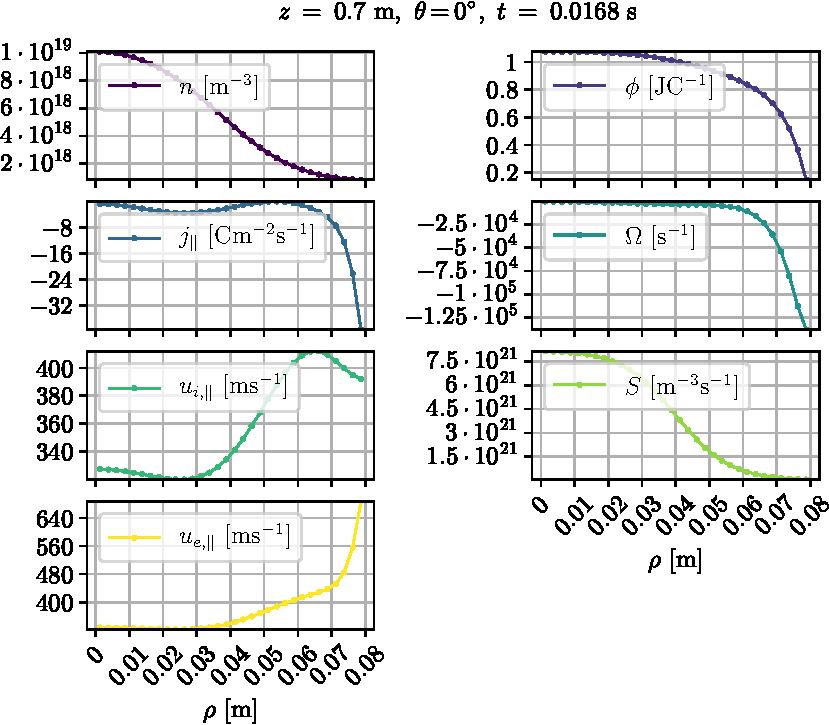
\includegraphics[width=1.0\textwidth]{fig/results/1DProfiles/B010Rad}
    \caption{Radial profiles in steady state for $B=0.1\T$}
    \label{fig:radProfs}
\end{figure}
%
The radial profiles are shown in \cref{fig:radProfs}.
As for the parallel direction, the shape of the radial density profile is determined mainly by the source and the radial boundary conditions.
The radial extent of the source plays a larger role in determining the radial density profile than the shape of the source.

Despite having almost Boltzmann distribution electrons in the parallel direction at each radial point close to the axis, the Boltzmann distribution not apply in the radial direction (due to the magnetic field).
Close to $L_\rho$ the radial potential profile is affected more by the fixation potential to $0$ at $L_\rho$.
The values here differs from the density profile because of the zero gradient enforcement on $n$ at $L_\rho$.

\section{The linear phase}
%
After perturbing the system as described in \cref{sec:initRun}, most of the noise vanishes and poloidal modes start to appear.
It has not been observed that the system reaches the linear phase unless perturbed.
This could in principle happen if the noise at machine level assembles in just the right way such that it forms an linearly unstable mode.
Depending on the simulation parameters, the poloidal modes will be damped to zero and the system will return to the steady state, or they will increase in amplitude.
As the perturbations are small, the dynamics in this linear phase come purely from the linear part of the set of equations.
In other words mode coupling between different modes are negligible.
Thus, if we were dealing with a purely linear system the growth of the modes would continue forever.
In any case, the modes are rotating either clockwise or counter clockwise (depending on the mode number and the simulation parameters), as indicated in \cref{fig:modeRotation}.

If one assumes that the perturbations are on the from $A\exp\L(i[k_\theta \theta - \L(i\Im[\om] + \Re[\om]\R) t]\R)$, one can assure oneself that positive $\Im(\om)$ causes exponential growth for increasing $t$, and a positive $\Re(\om)$ causes a counter-clockwise rotation of the perturbation (given that $\theta$ grows in the counter-clockwise direction) as the inverse wavelength $k_\theta$ stays constant.
%
% FIXME; Could add arrow indicating direction of rotation
%
\begin{figure}[htbp]
    \centering
    \begin{subfigure}[h]{1.00\textwidth}
        \centering
        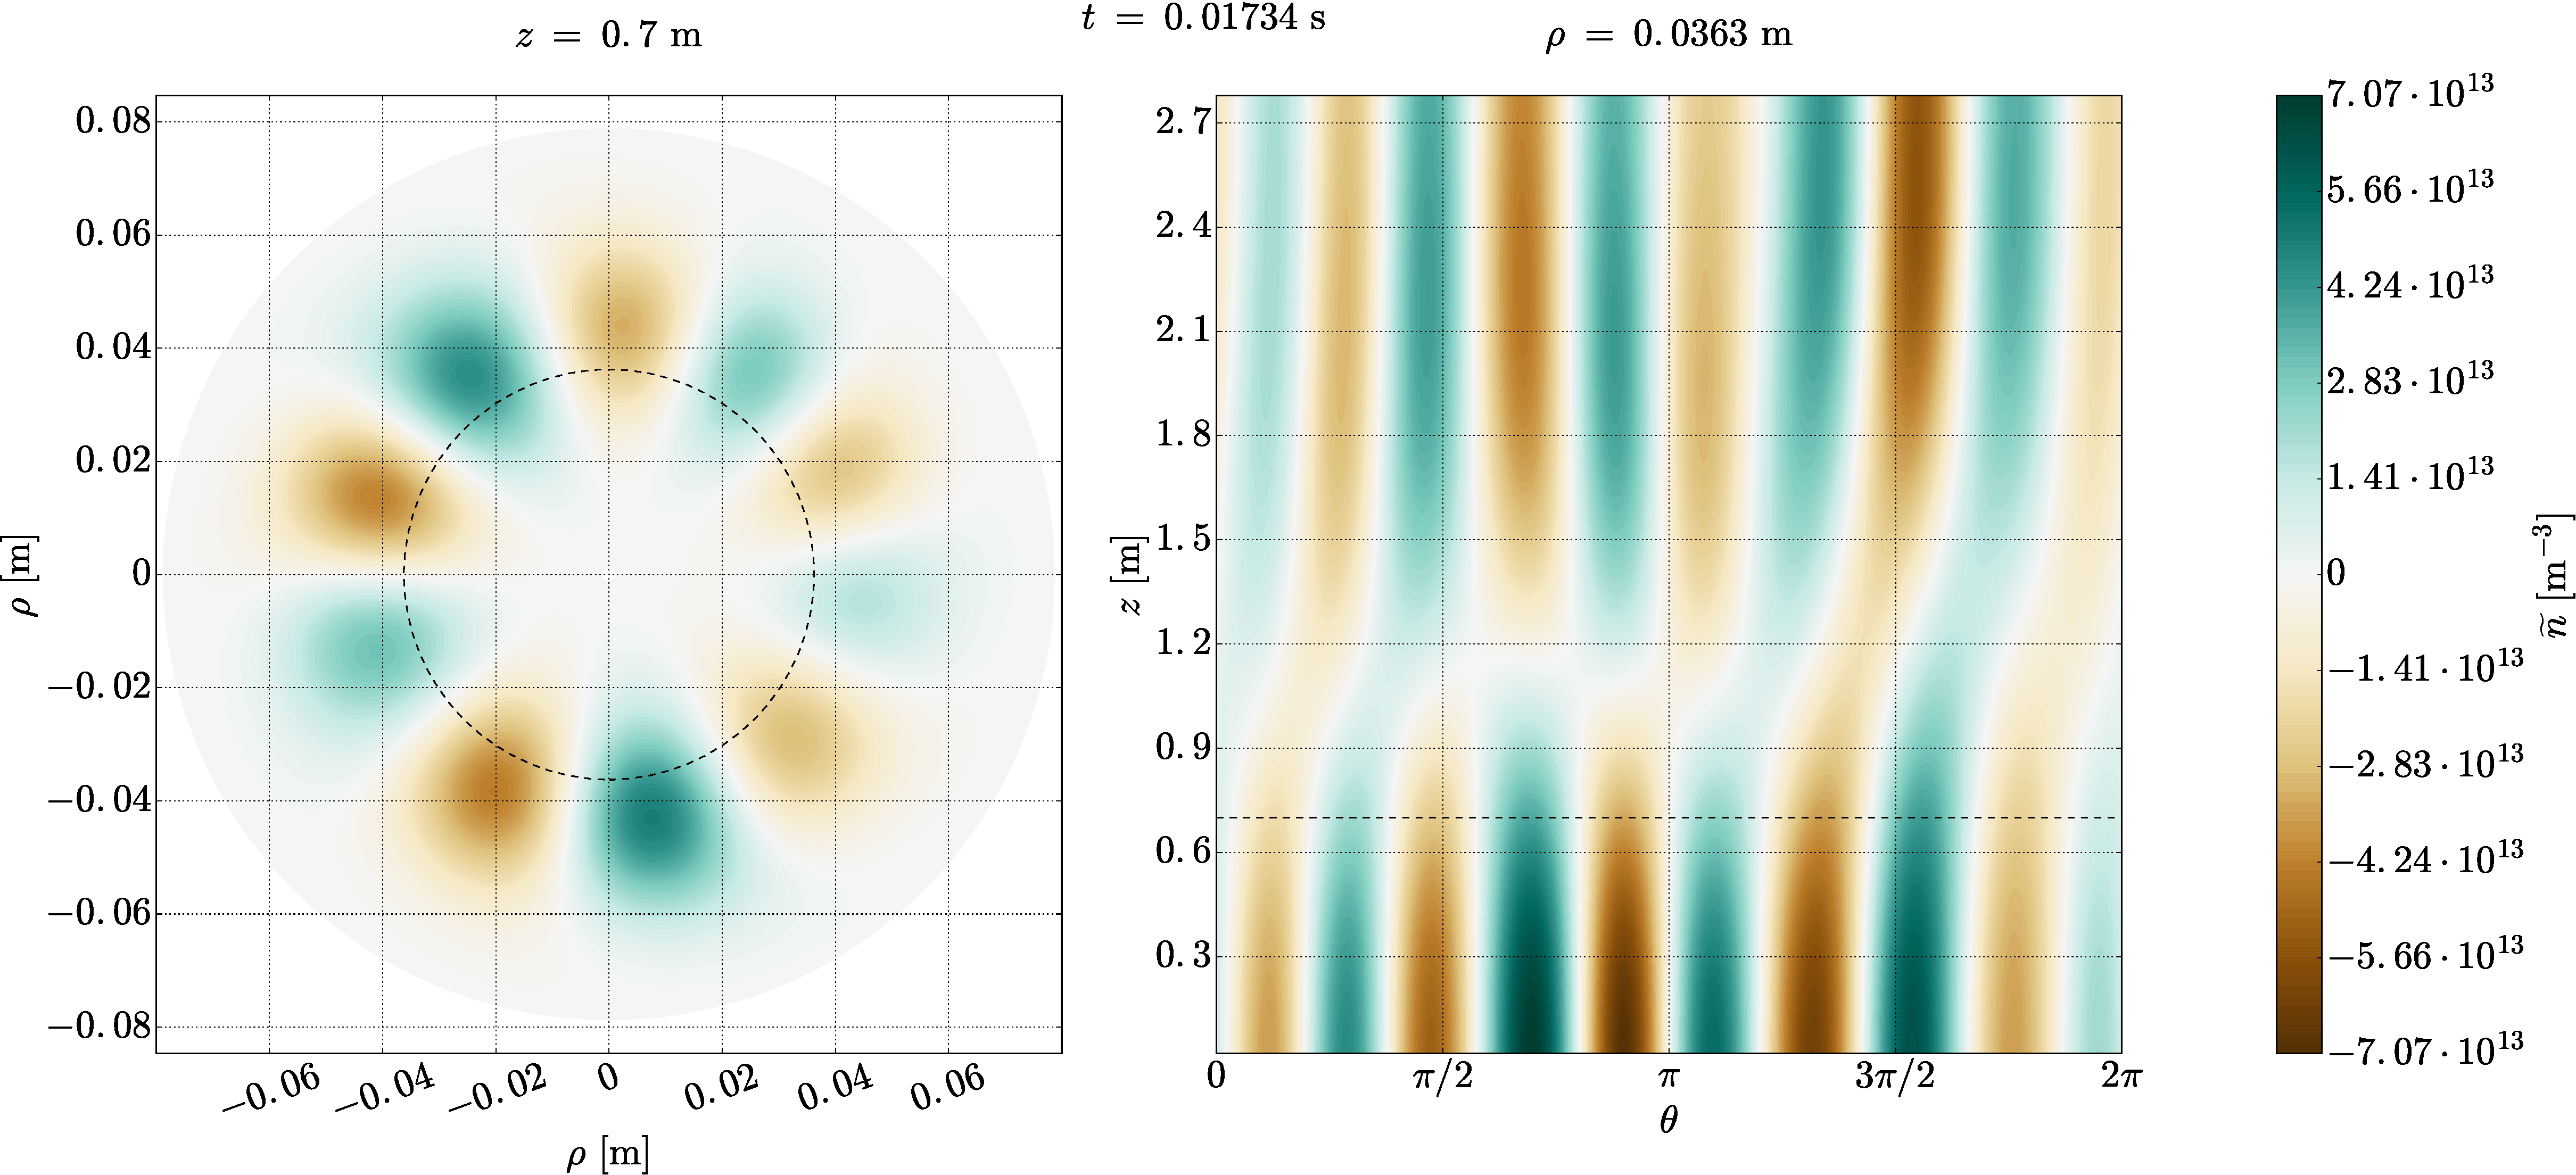
\includegraphics[width=1.0\textwidth]{fig/results/rotModes/n-perpPol-2D-fluct-0}
        \label{fig:rot1}
    \end{subfigure}%
    \\
    \begin{subfigure}[h]{1.00\textwidth}
        \centering
        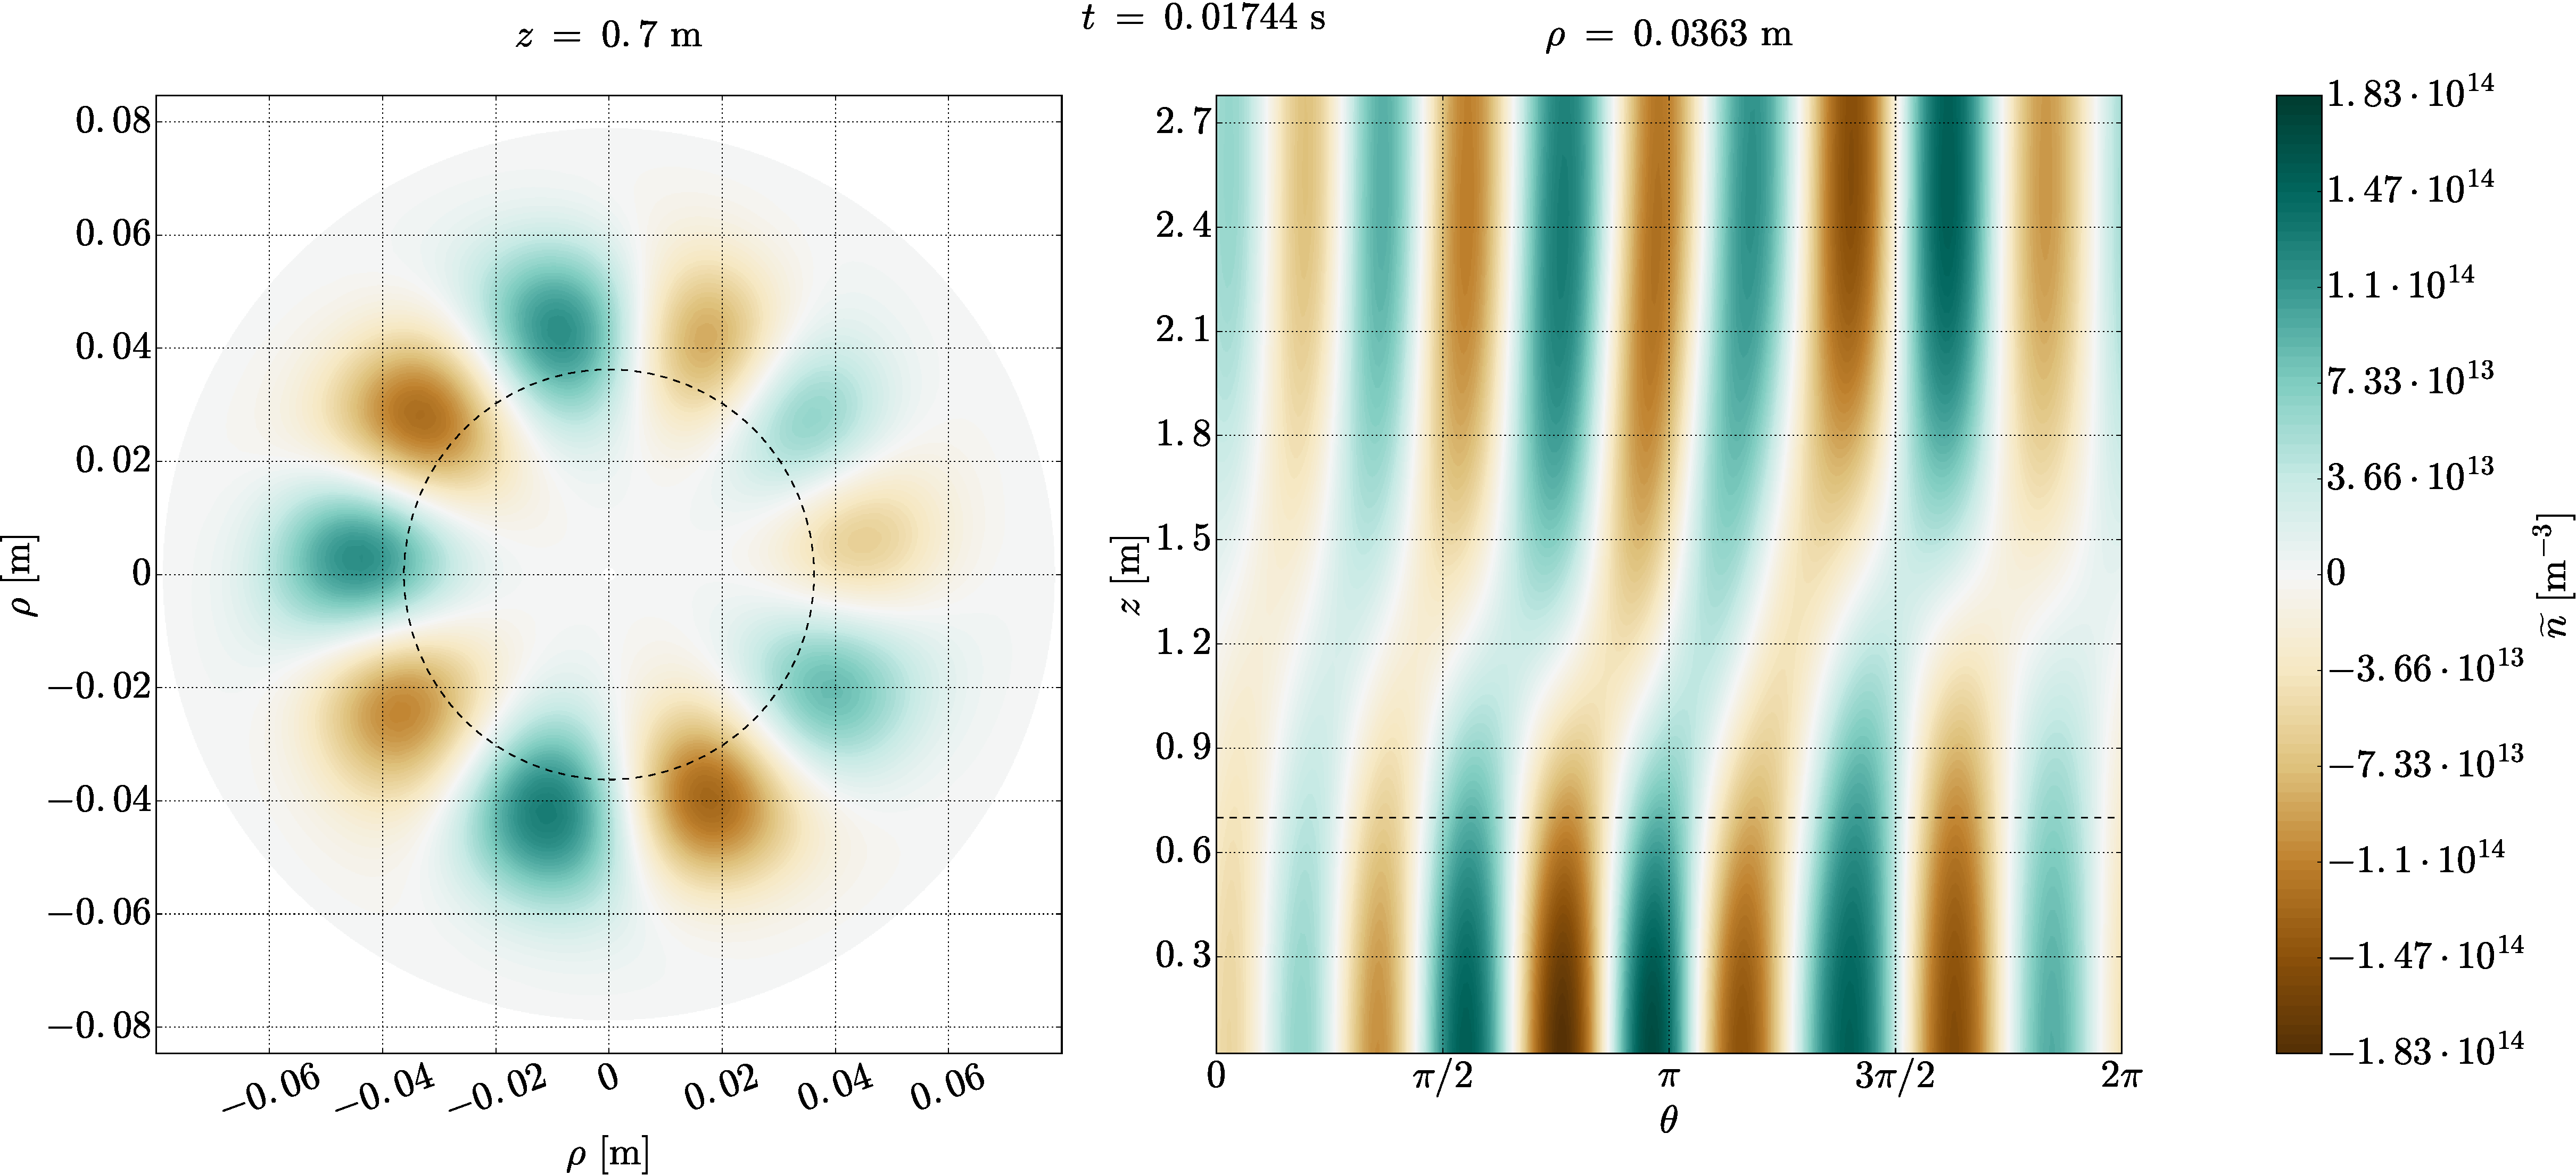
\includegraphics[width=1.0\textwidth]{fig/results/rotModes/n-perpPol-2D-fluct-1}
        \label{fig:rot2}
    \end{subfigure}
    \\
    \begin{subfigure}[h]{1.00\textwidth}
        \centering
        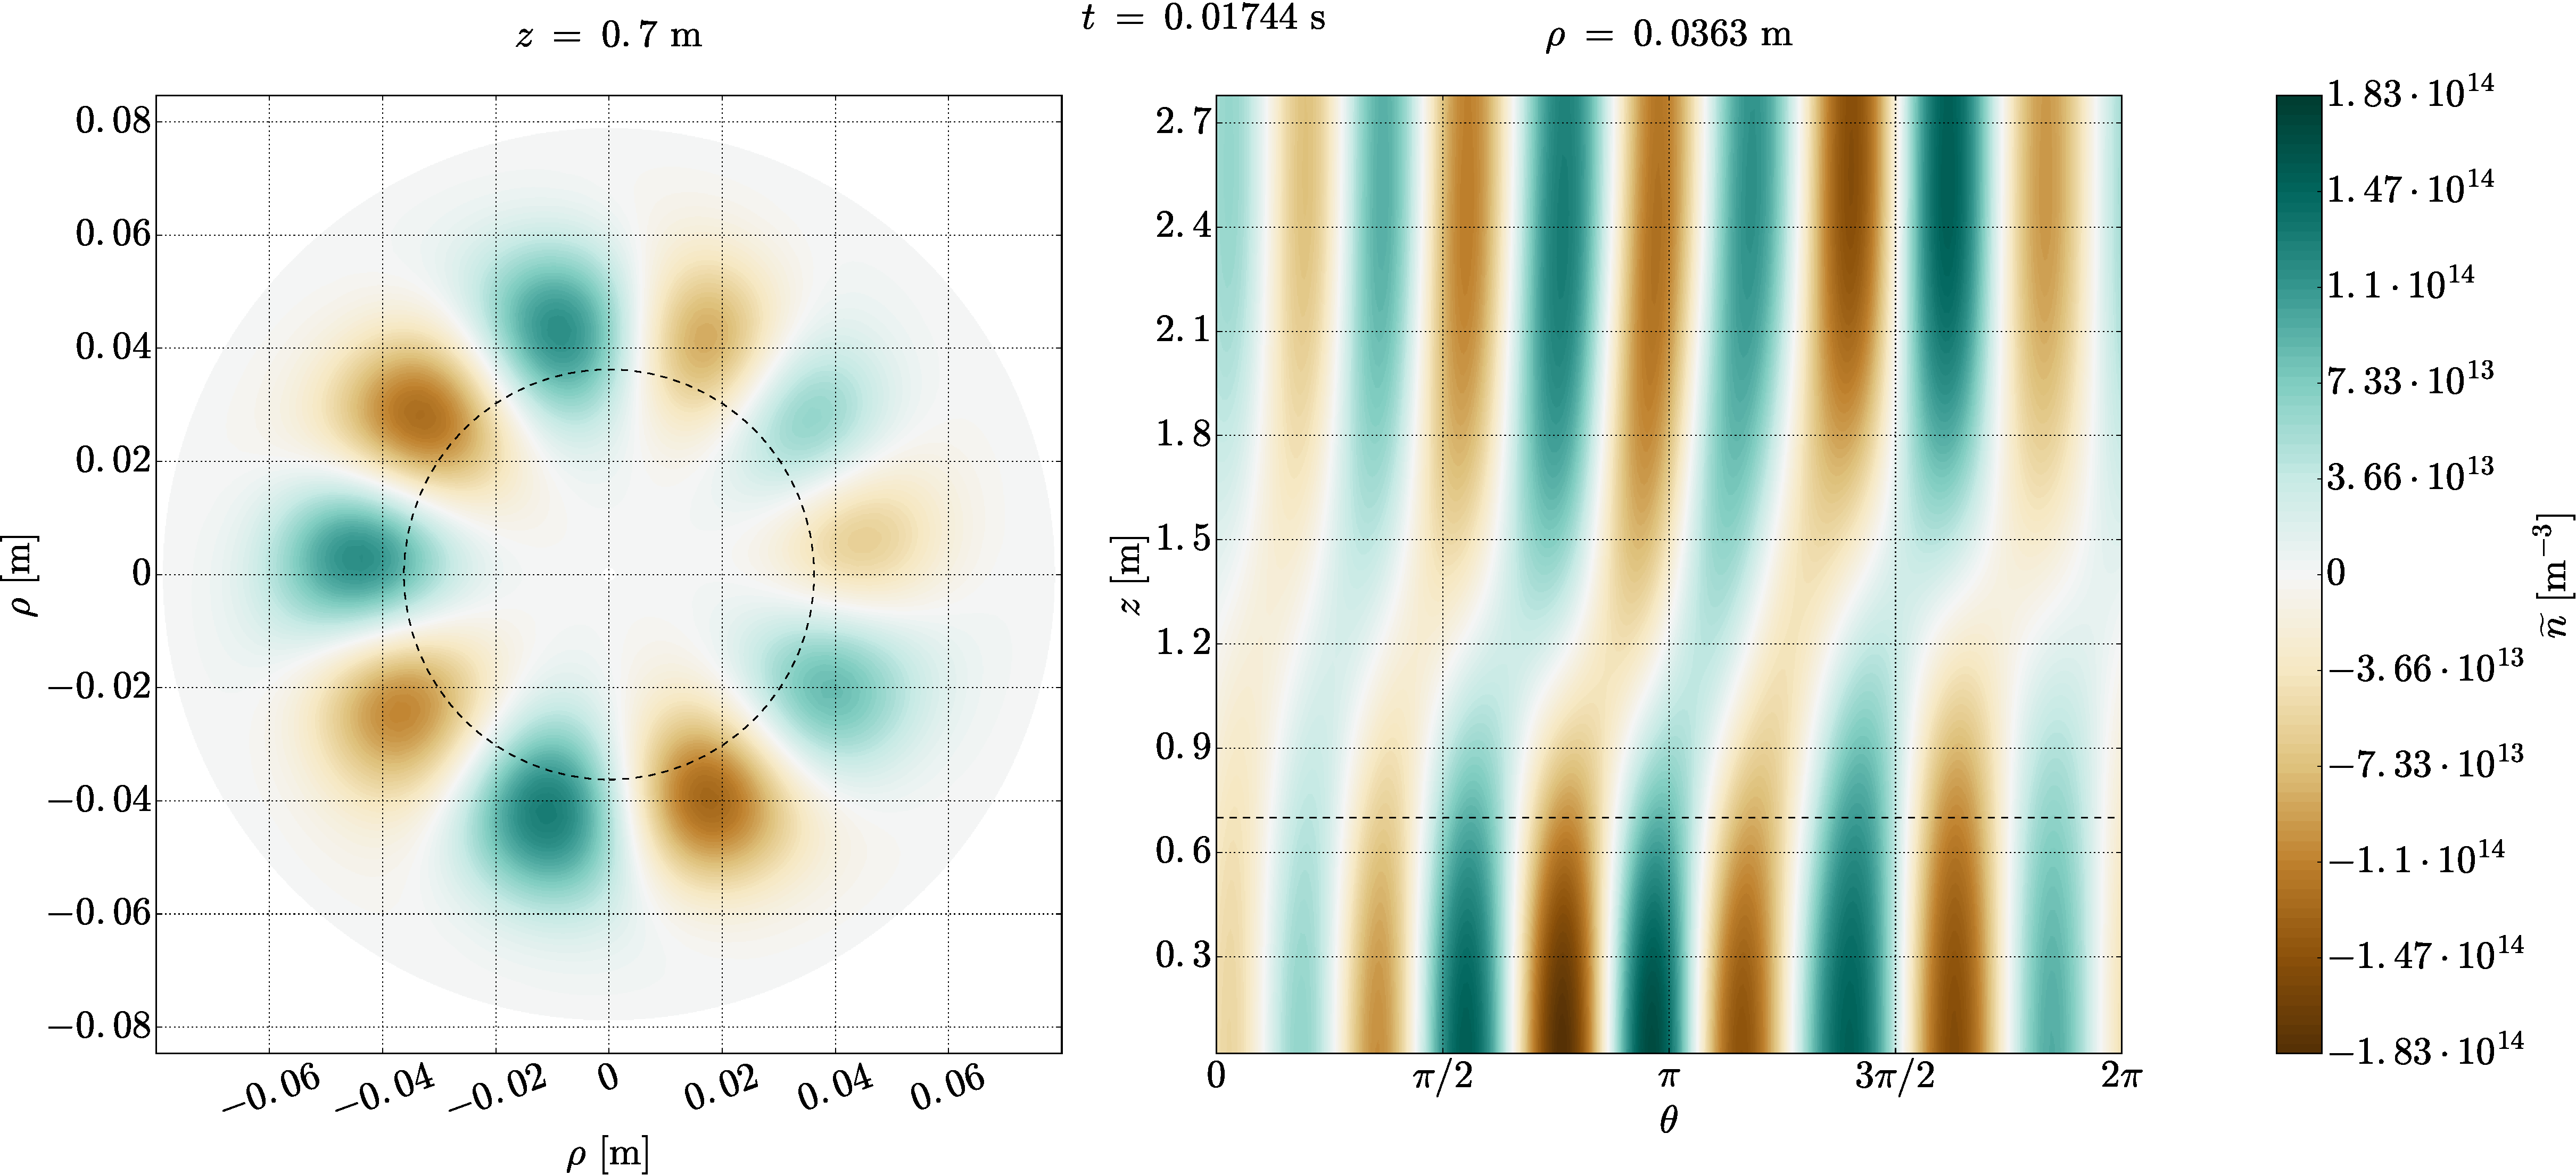
\includegraphics[width=1.0\textwidth]{fig/results/rotModes/n-perpPol-2D-fluct-2}
        \label{fig:rot3}
    \end{subfigure}
    \caption{Rotation of modes}
    \label{fig:modeRotation}
\end{figure}
%
Which poloidal mode which will dominate is dependent on $B$.
This is depicted in \cref{fig:dominatingMode}.
%
\begin{figure}[htbp]
    \centering
    \begin{subfigure}[h]{1.00\textwidth}
        \centering
        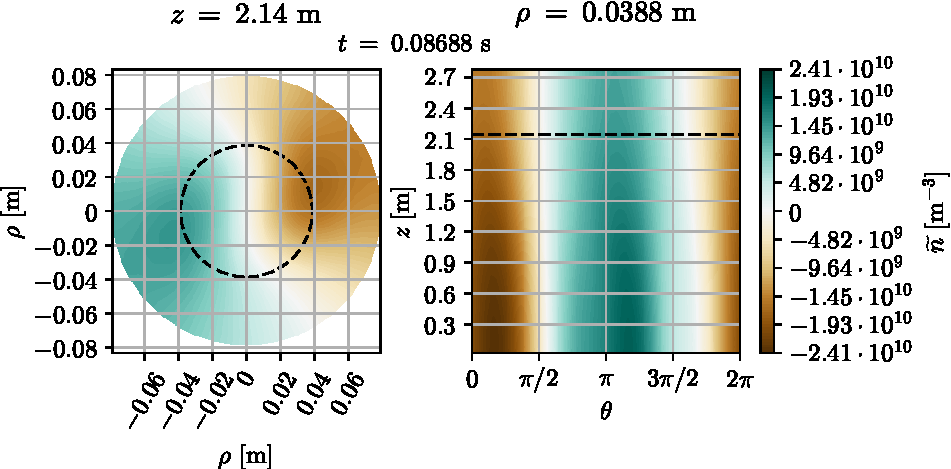
\includegraphics[width=1.0\textwidth]{fig/results/modesDiffScanVals/B002}
        \caption{$B=0.02 \T$}
        \label{fig:B002}
    \end{subfigure}%
    \\
    \begin{subfigure}[h]{1.00\textwidth}
        \centering
        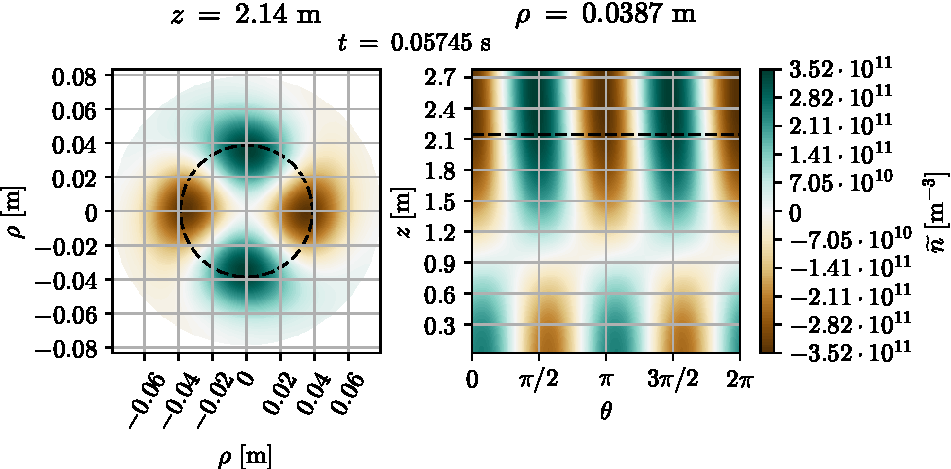
\includegraphics[width=1.0\textwidth]{fig/results/modesDiffScanVals/B004}
        \caption{$B=0.04 \T$}
        \label{fig:B004}
    \end{subfigure}
    \\
    \begin{subfigure}[h]{1.00\textwidth}
        \centering
        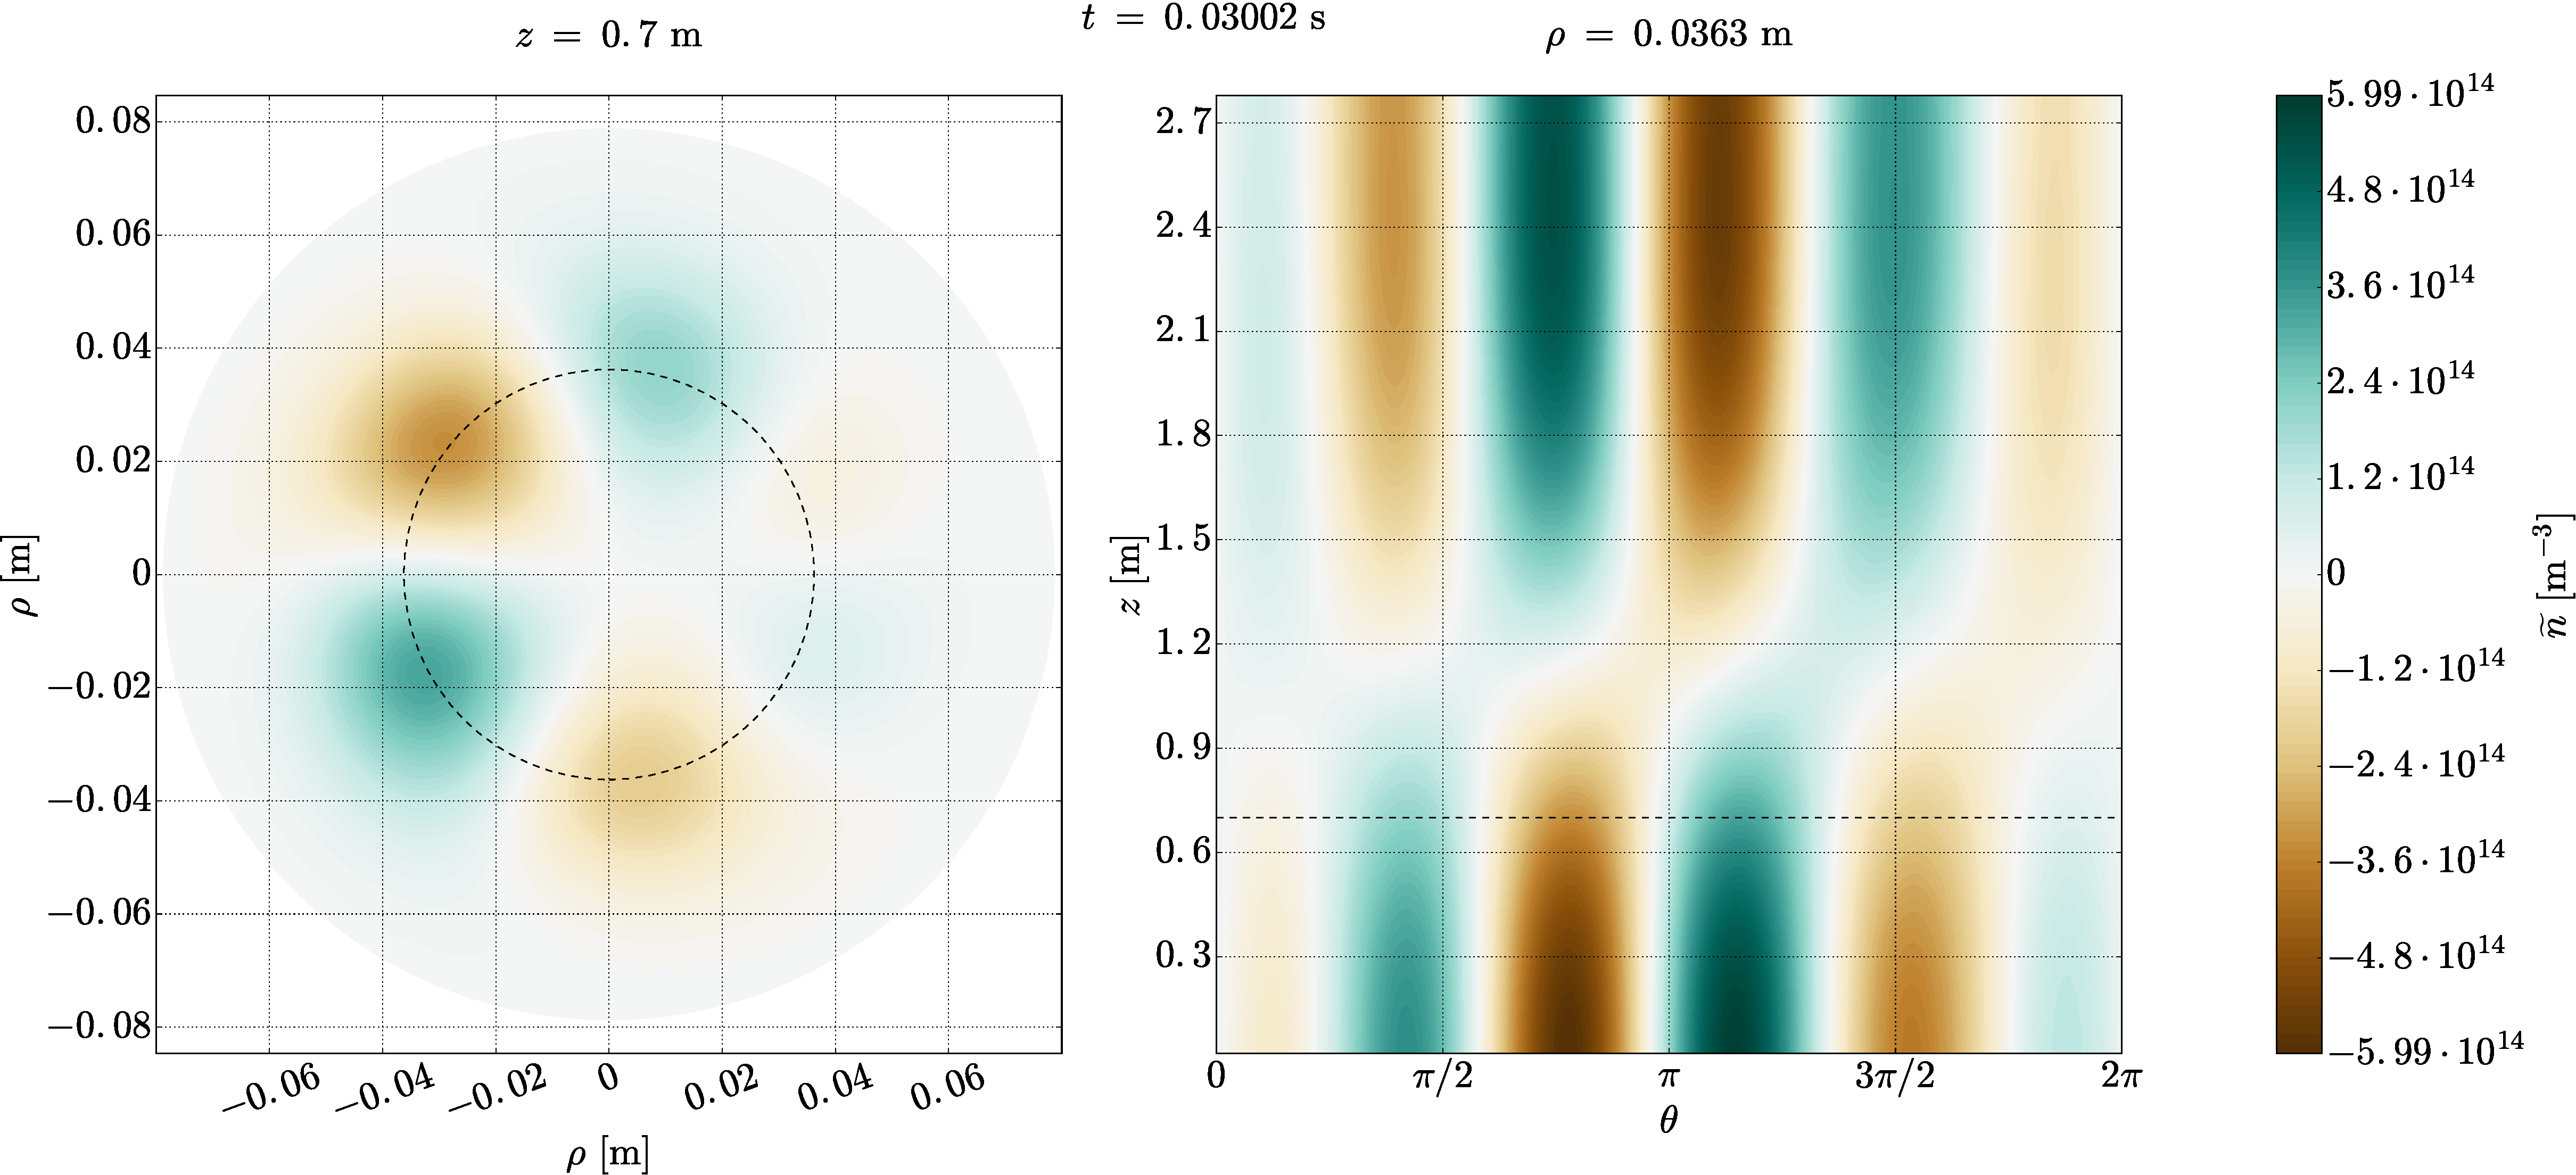
\includegraphics[width=1.0\textwidth]{fig/results/modesDiffScanVals/B006}
        \caption{$B=0.06 \T$}
        \label{fig:B006}
    \end{subfigure}
    \caption{Dominant mode depends on $B$}
    \label{fig:dominatingMode}
\end{figure}
%
One can also note that the parallel node moves downward with decreasing $B$.

A more quantitative way to look at the linear phase is to plot the Fourier modes at the position of the most unstable growth.
From linear stability theory (FIXME)
% FIXME: Add references
, the position of the most unstable mode for drift waves coincides with the position of largest gradient.
The modes are depicted in \cref{fig:fourierDens}.
As the abscissa is logarithmic, exponential grow will appear as straight lines.
%
\begin{figure}[h!]
    \centering
    \begin{subfigure}[h]{0.45\textwidth}
        \centering
        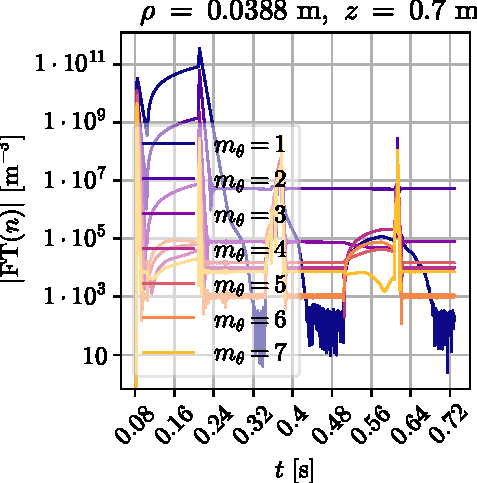
\includegraphics[width=1.0\textwidth]{fig/results/fourierModes/stable}
        \label{fig:fourierStable}
        \caption{For $B=0.02\T$ the system is stable against perturbation}
    \end{subfigure}%
    \hfill
    \begin{subfigure}[h]{0.45\textwidth}
        \centering
        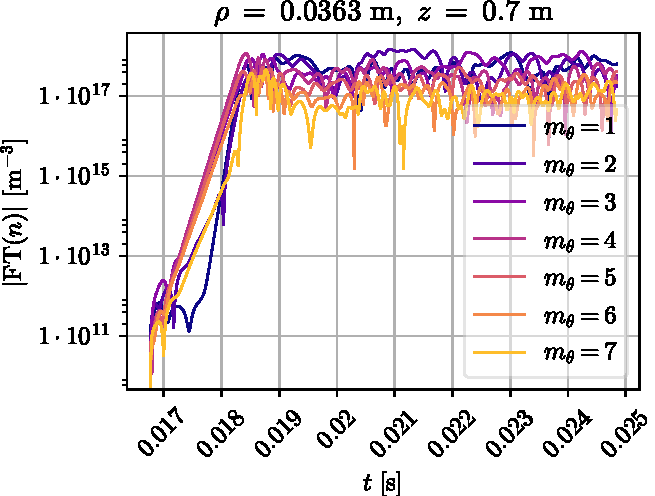
\includegraphics[width=1.0\textwidth]{fig/results/fourierModes/unstable}
        \label{fig:fourierUnstable}
        \caption{Growth rate leading to saturated turbulence for $B=0.1\T$}
    \end{subfigure}
    \caption{Time trace of the absolute values of the Fourier modes.}
    \label{fig:fourierDens}
\end{figure}
%
The slope of the absolute values of the Fourier modes gives us the growth rate, whereas the angular velocity can be found from
%
\begin{align*}
    \Re[\om_n(t)] =
    \frac{
        \frac{\Im[\text{FT}(n[t_1])]}{\Re[\text{FT}(n[t_1])]} -
        \frac{\Im[\text{FT}(n[t_0])]}{\Re[\text{FT}(n[t_0])]}
    }{\Delta t}
\end{align*}
%
where $\text{FT}$ denotes the Fourier transformed.
The final angular velocity is the average of the individual angular velocities of the linear phase, where the start and the end of the linear phase has been determined by visual inspection.
The start has been defined as the time where the initial perturbation has vanished, and where the modes start to show a more or less exponential growth.
The end is defined as the time where any mode, which up to that point in time has been flat or damped suddenly shows an exponential growth.
\Cref{fig:gr} depicts the $B$ dependencies on the growth rates.
%
\begin{figure}[htb]
    \centering
    \begin{subfigure}[h]{1.00\textwidth}
        \centering
        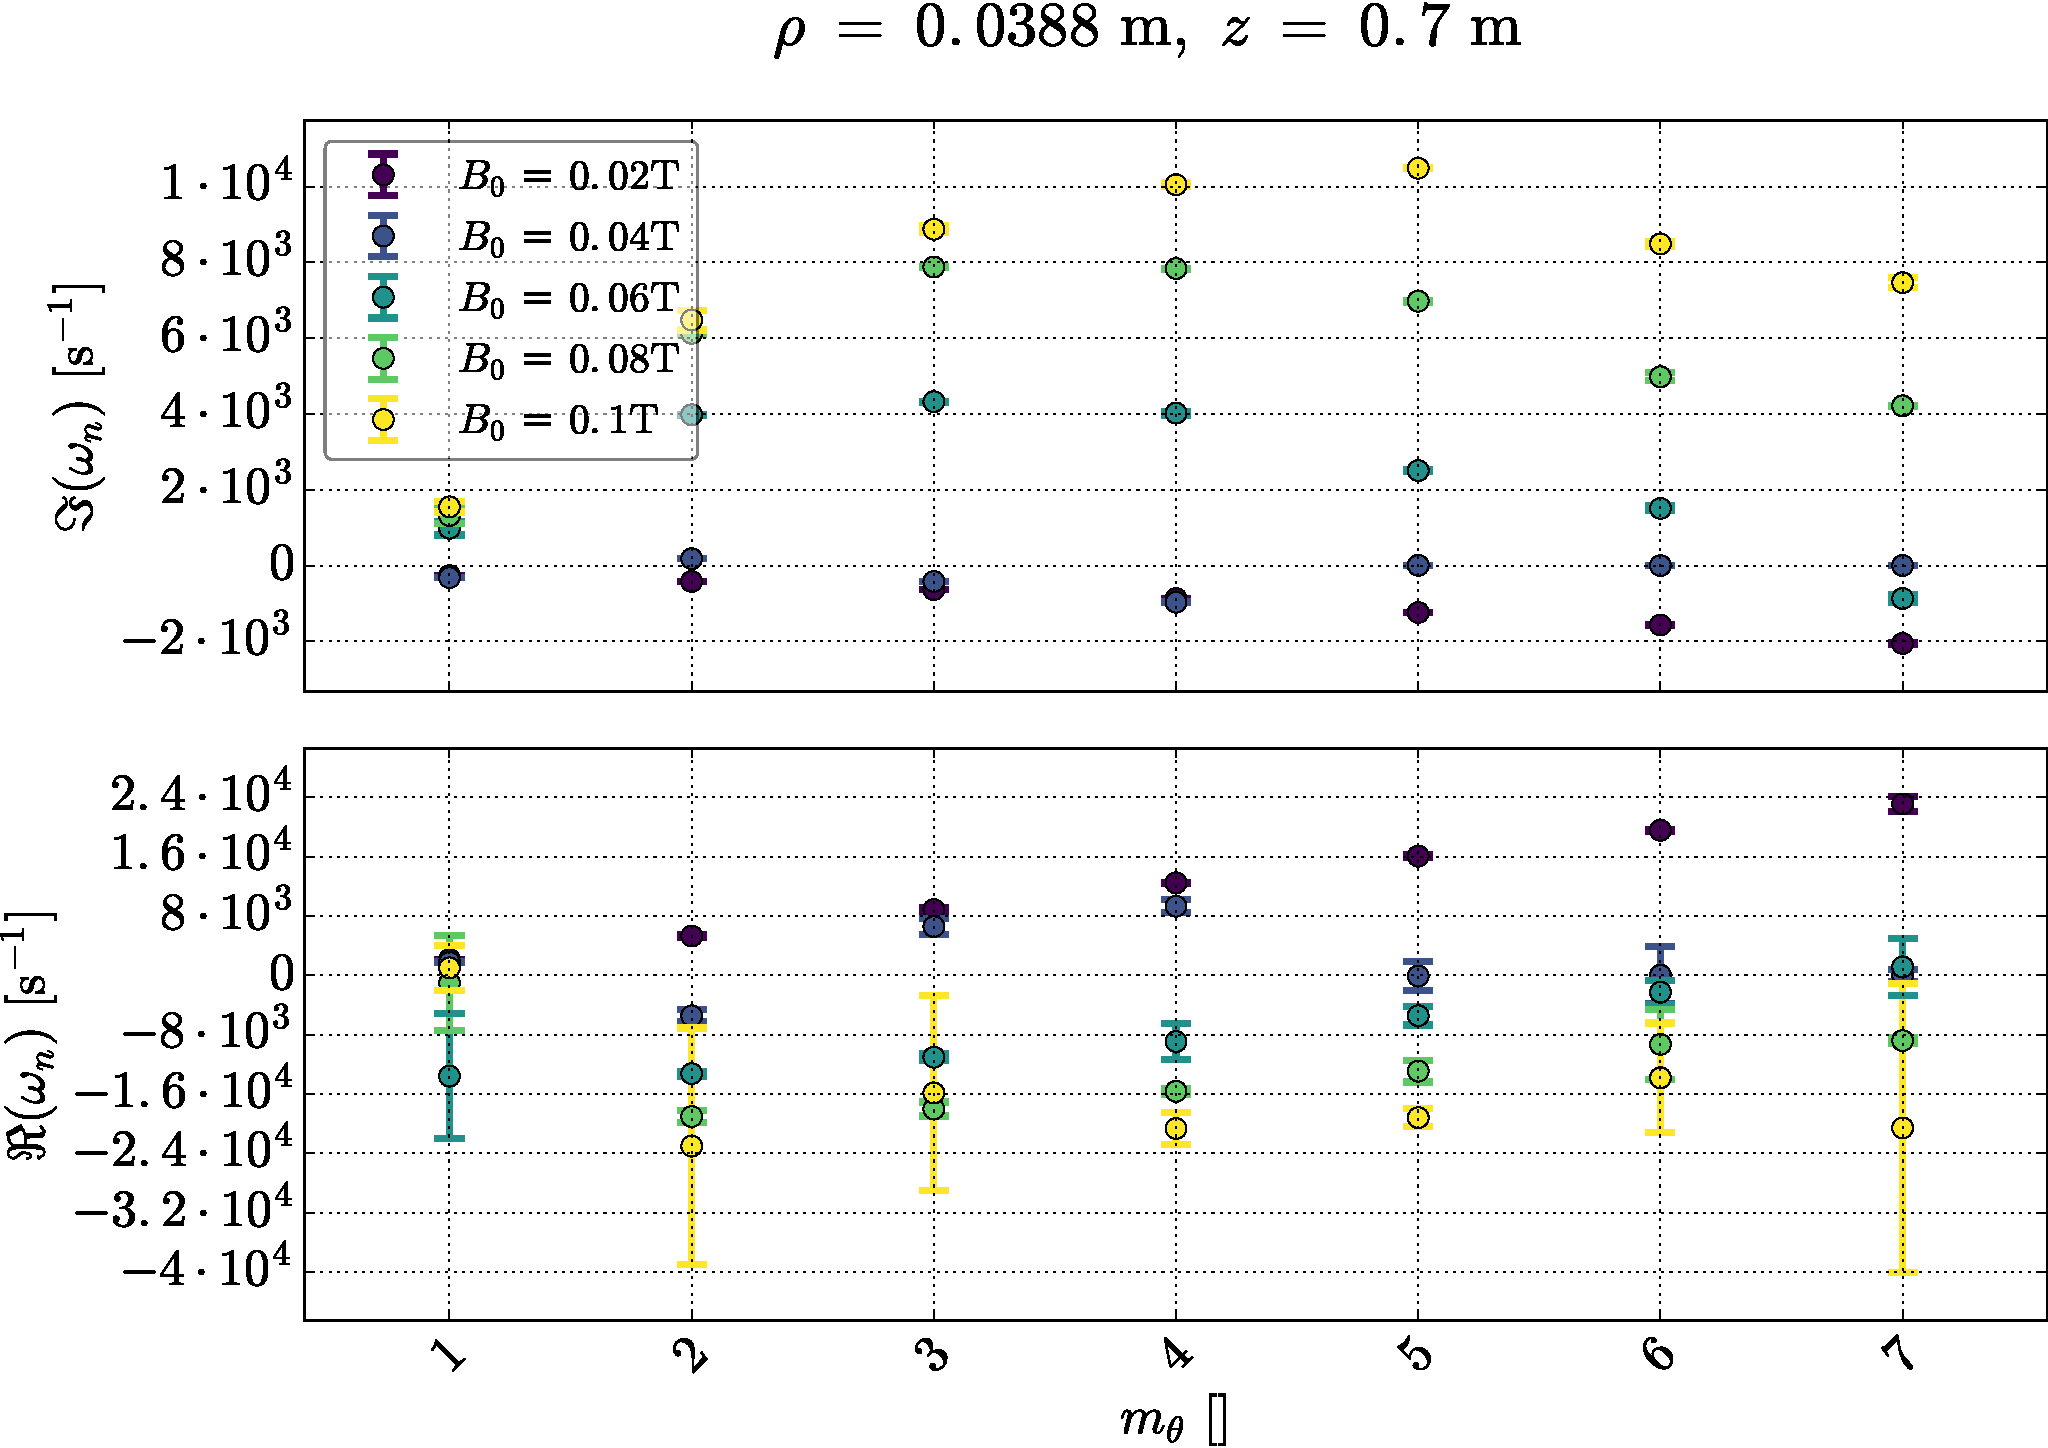
\includegraphics[width=1.0\textwidth]{fig/results/growthRates/growthRatesB0}
        \label{fig:grB}
    \end{subfigure}%
    \\
    \begin{subfigure}[h]{1.00\textwidth}
        \centering
        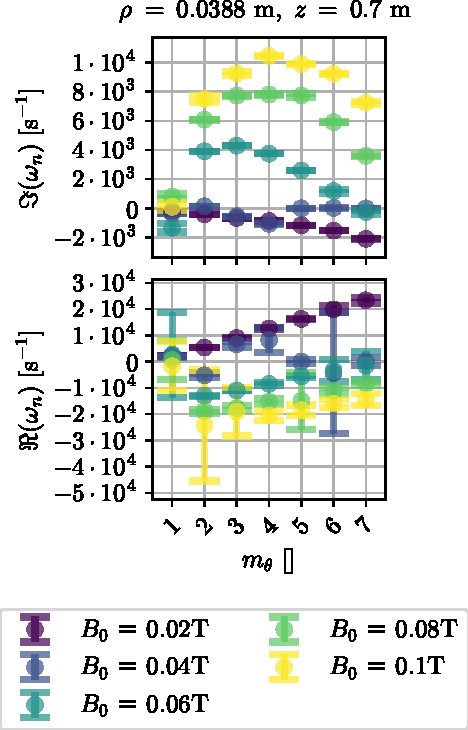
\includegraphics[width=1.0\textwidth]{fig/results/growthRates/growthRatesB0ModeNr}
        \label{fig:grBModeNr}
    \end{subfigure}
    \caption{$B$-dependency on the growth rates and angular velocities.}
    \label{fig:gr}
\end{figure}
%
% FIXME: Explain why compare is different?

FIXME: Compare gr with analytic gr.

FIXME: Figures are scattered all over.

\section{The turbulence phase}
%
At a certain point the linear modes becomes large enough for non-linear effects to affect the dynamics of the system.
Through the non-linearities in the equation, mode-mode coupling occurs, leading to a cascading of enstrophy (global integrated vorticity) and energy.
The radial displacement of fluid parcels is much more restricted than the displacement along the field lines due to the magnetic field.
Consequently, the turbulence cascade have a more a 2 dimensional character than a 3 dimensional character.
In 2-D turbulence there is an inverse cascade of enstrophy as vortex stretching cannot occur.
In other words eddies tend to merge together to larger coherent structures.
This is something which is also seen in atmospheric flows, such as for example the great red spot on Jupiter.

FIXME: Back this up with references etc.

The main part of the energy is still cascading towards the smaller structures in 2-D turbulence.
At small enough scales the energy dissipates through diffusive processes.
The turbulence will reach a steady state once the input of energy through the source is balanced by the dissipation of energy.
On the transition from the linear phase to the turbulent phase a energy overshot is observed as seen in \cref{fig:energyTrace008}.
%
\begin{figure}[htb]
    \centering
    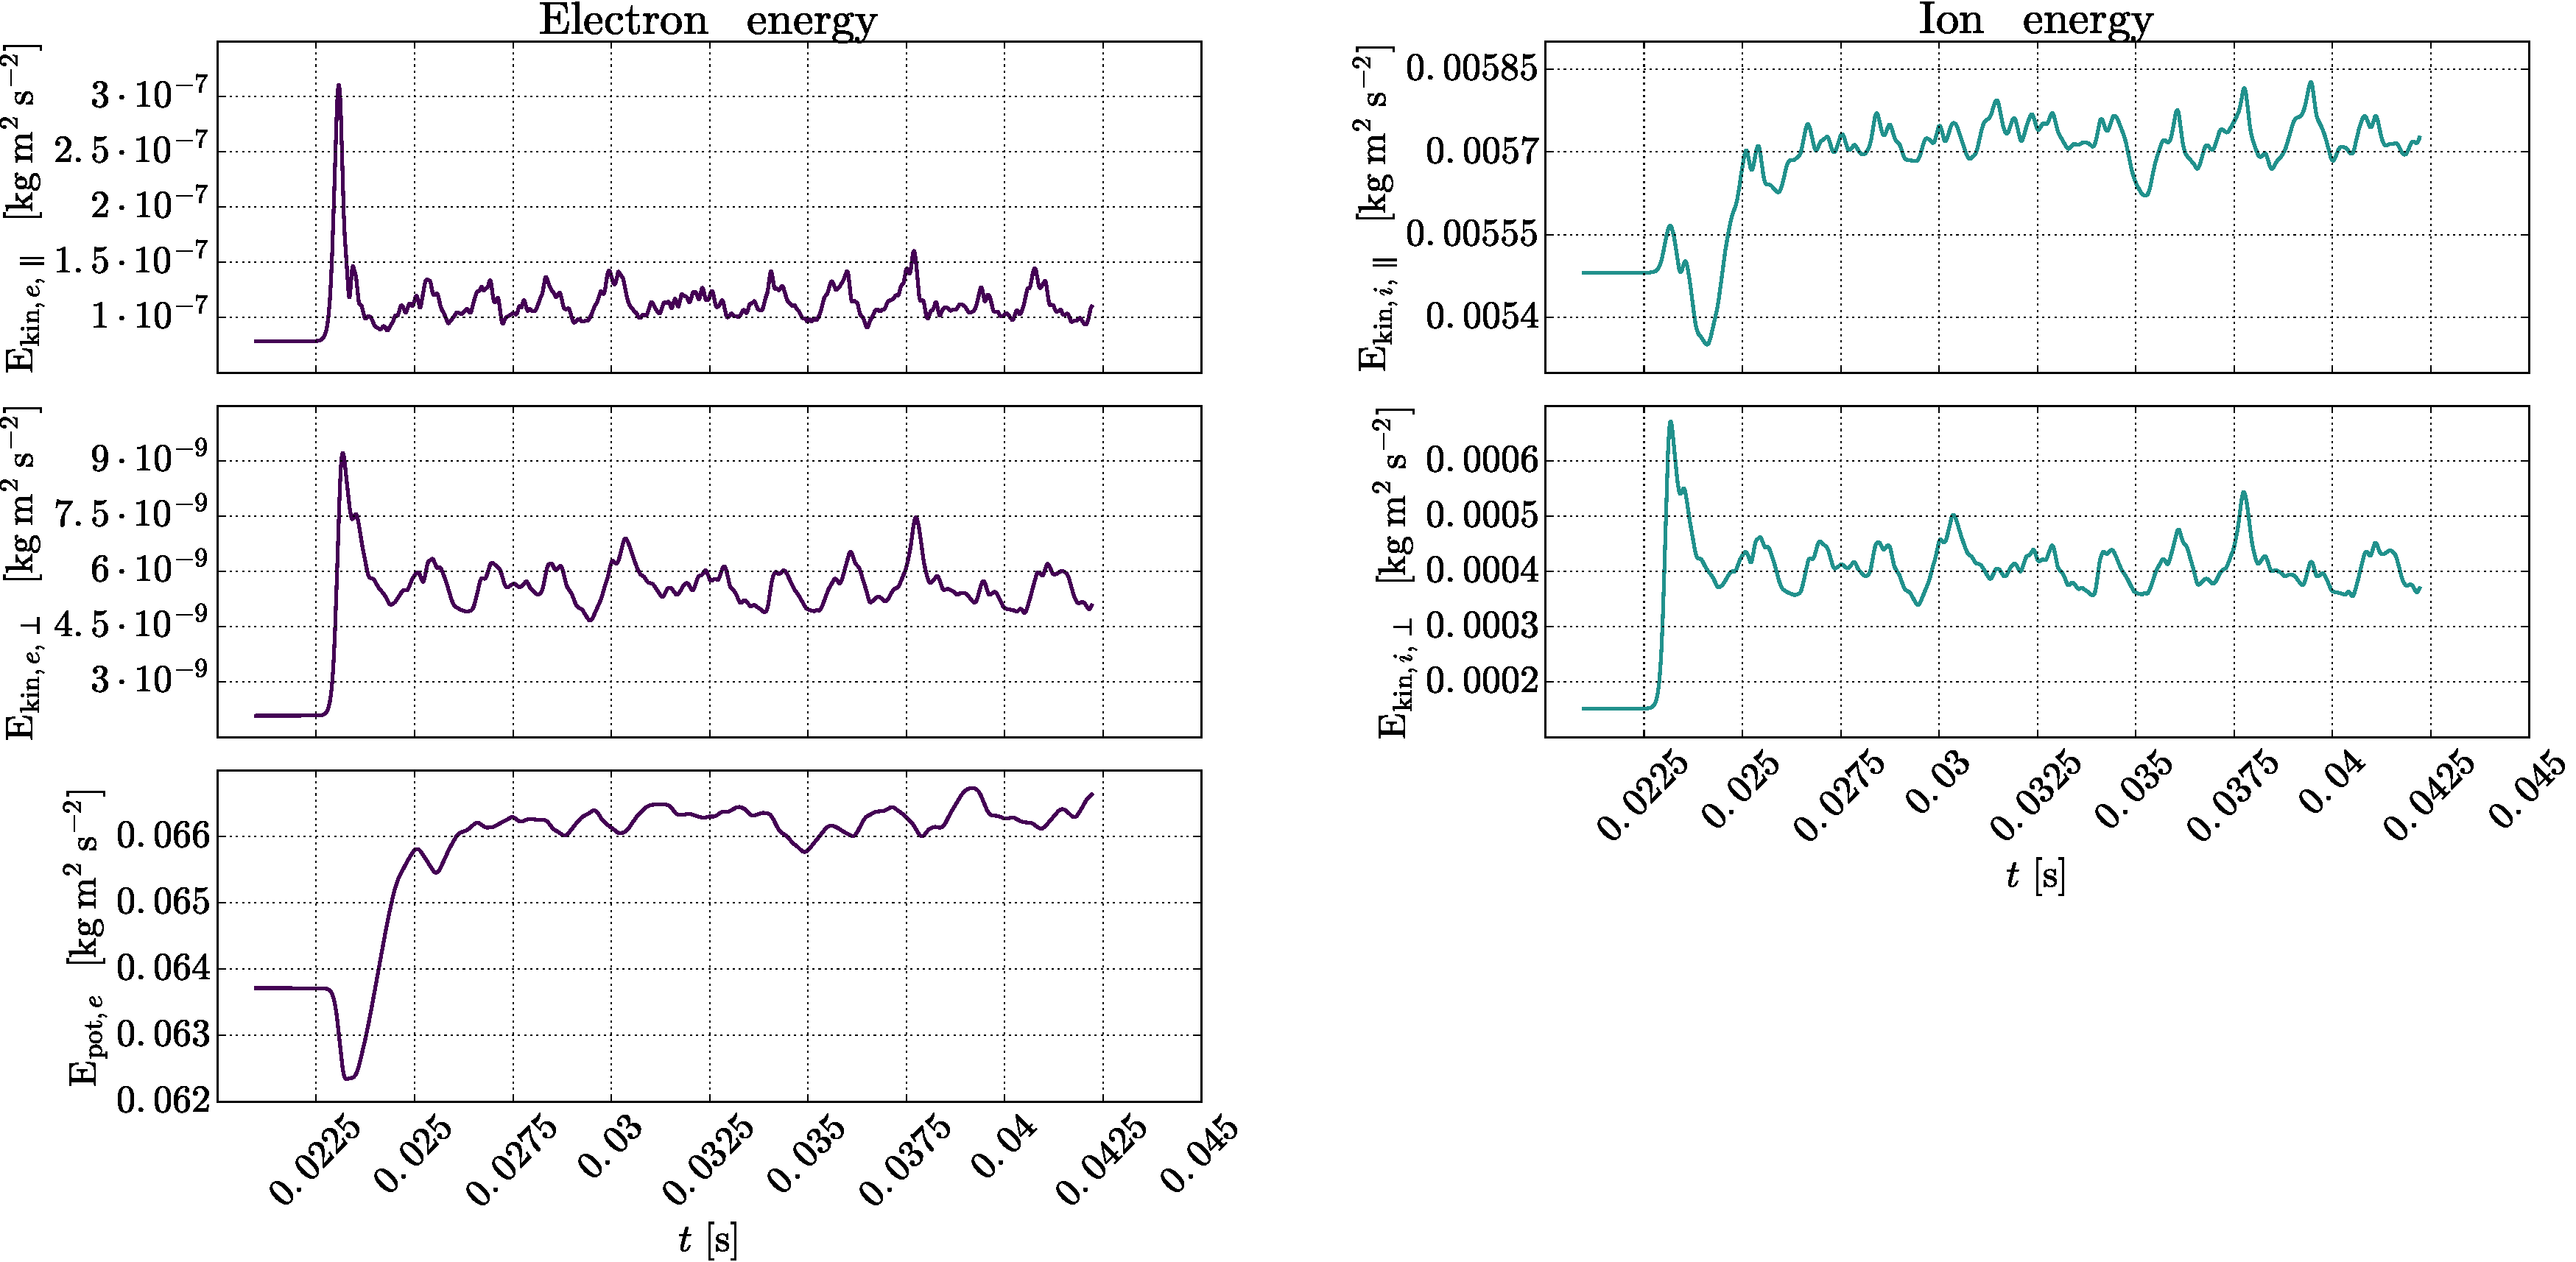
\includegraphics[width=1.0\textwidth]{fig/results/energyTrace/energyTraceB008}
    \caption{Time trace of the energy for $B=0.08$.}
    \label{fig:energyTrace008}
\end{figure}

As a consequence the eddies evolve at a faster phase at the transition as compared with the saturated turbulent state where eddies evolve at a slower rate.
In the saturated state the energy stays closer to the temporal mean, shown in \cref{fig:energyTrace008}.
It is also important to observe that the fluctuations can be big enough to push the plasma off center as observed in \cref{fig:offcenter}.
%
\begin{figure}[htbp]
    \centering
    \begin{subfigure}[h]{1.00\textwidth}
        \centering
        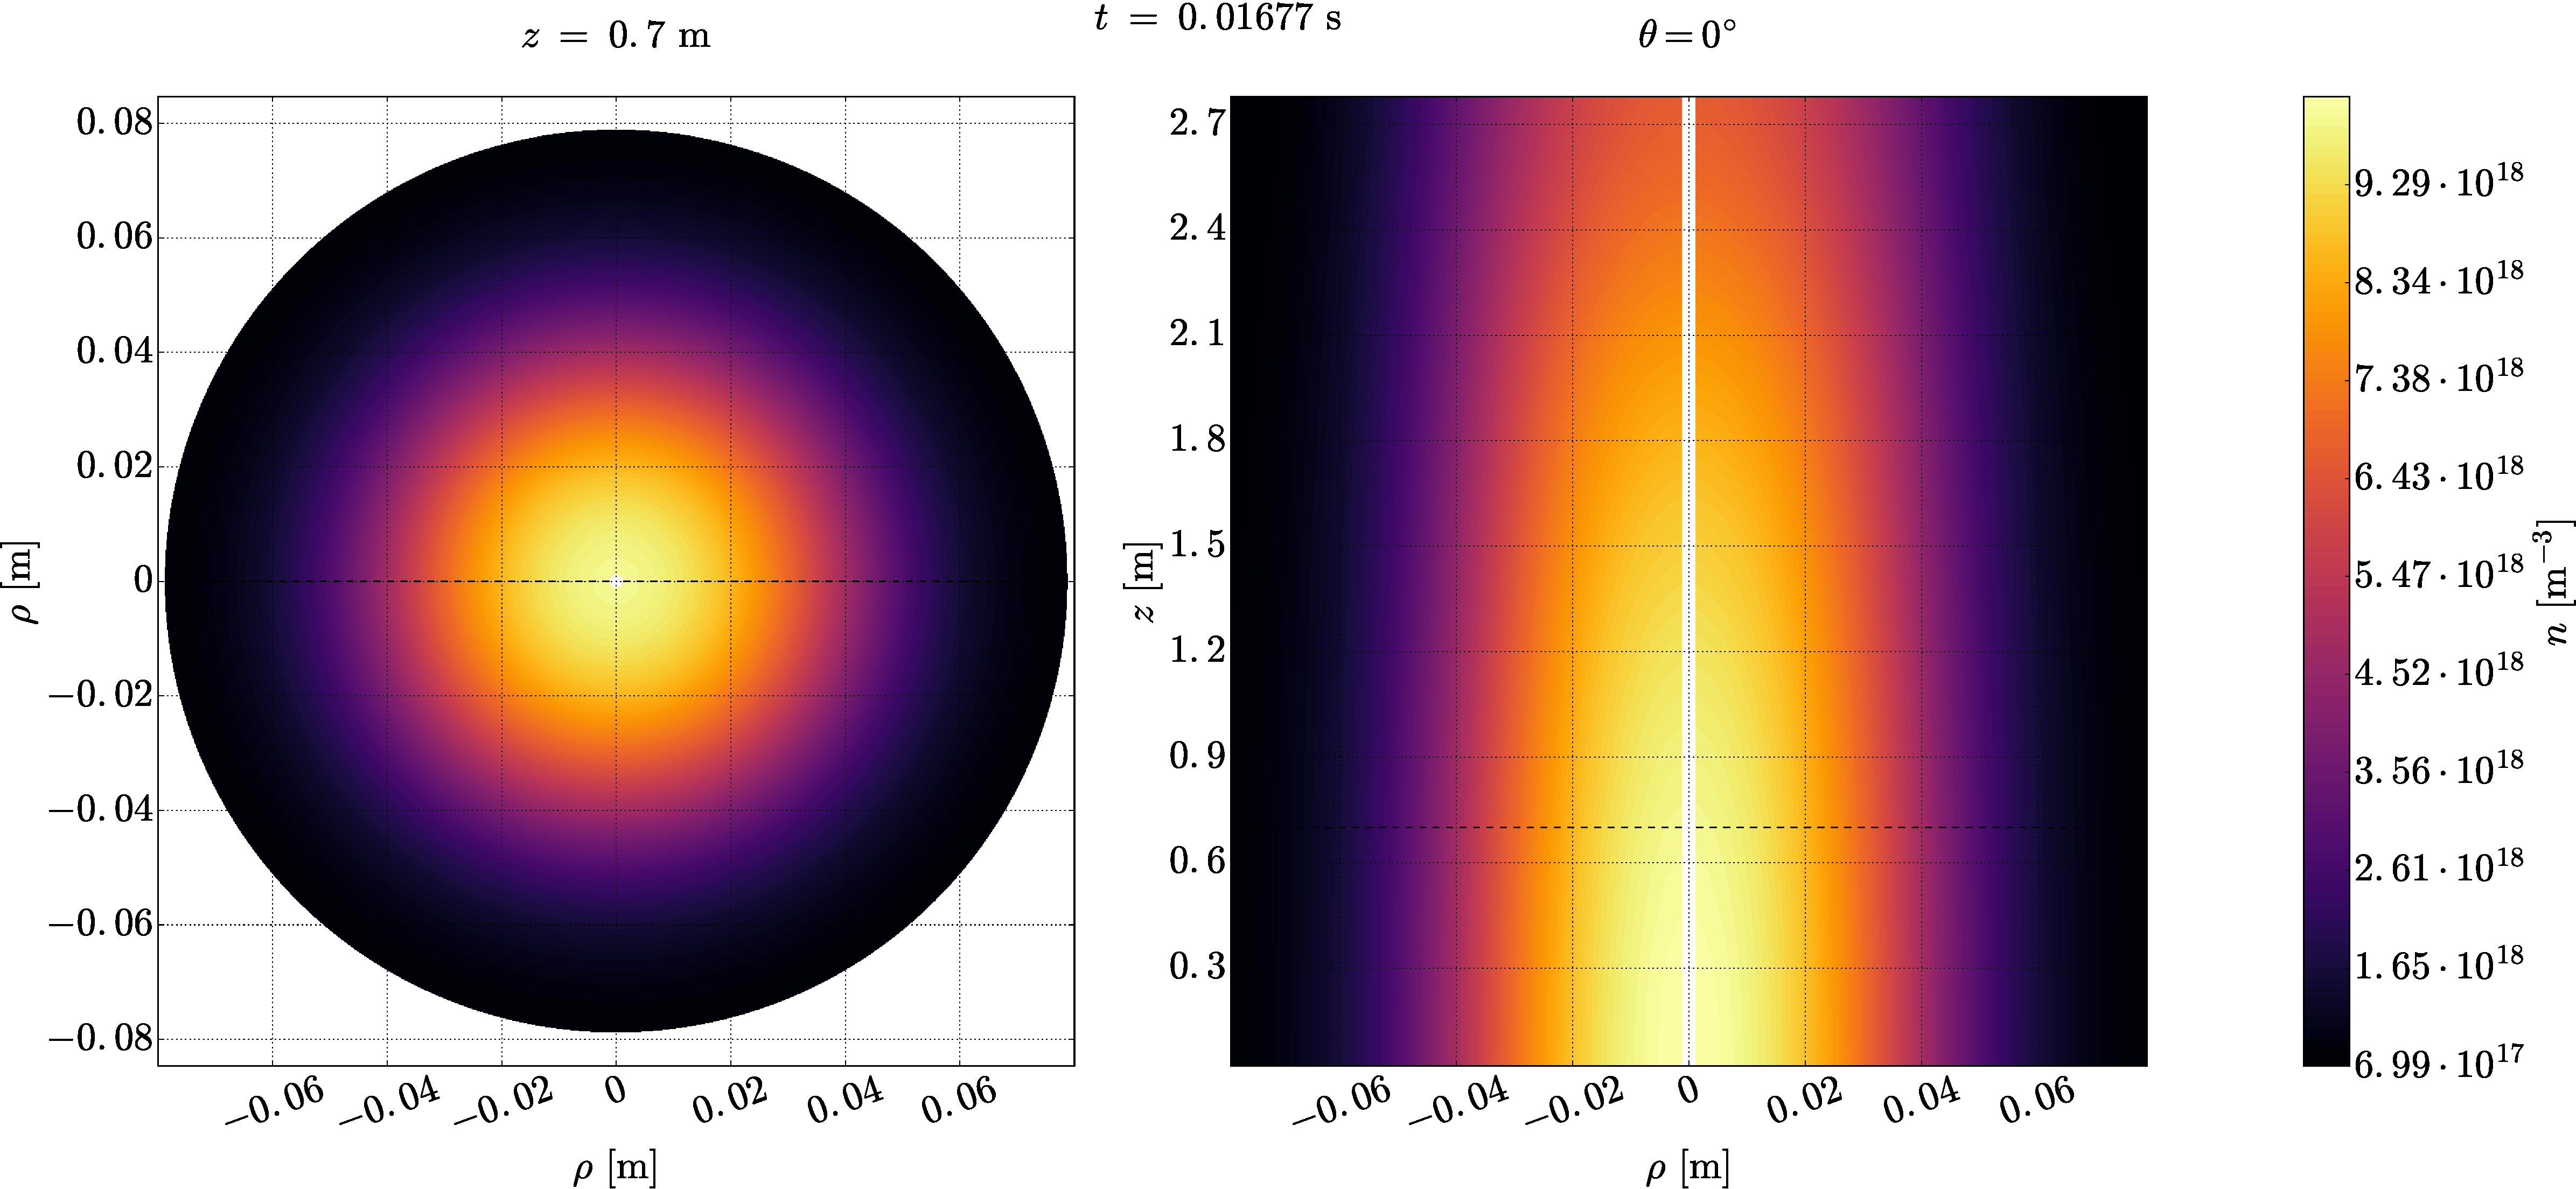
\includegraphics[width=1.0\textwidth]{fig/results/2DTurbulence/steadyStateN}
        \caption{The plasma at the steady state.}
        \label{fig:2Dsteady}
    \end{subfigure}%
    \\
    \begin{subfigure}[h]{1.00\textwidth}
        \centering
        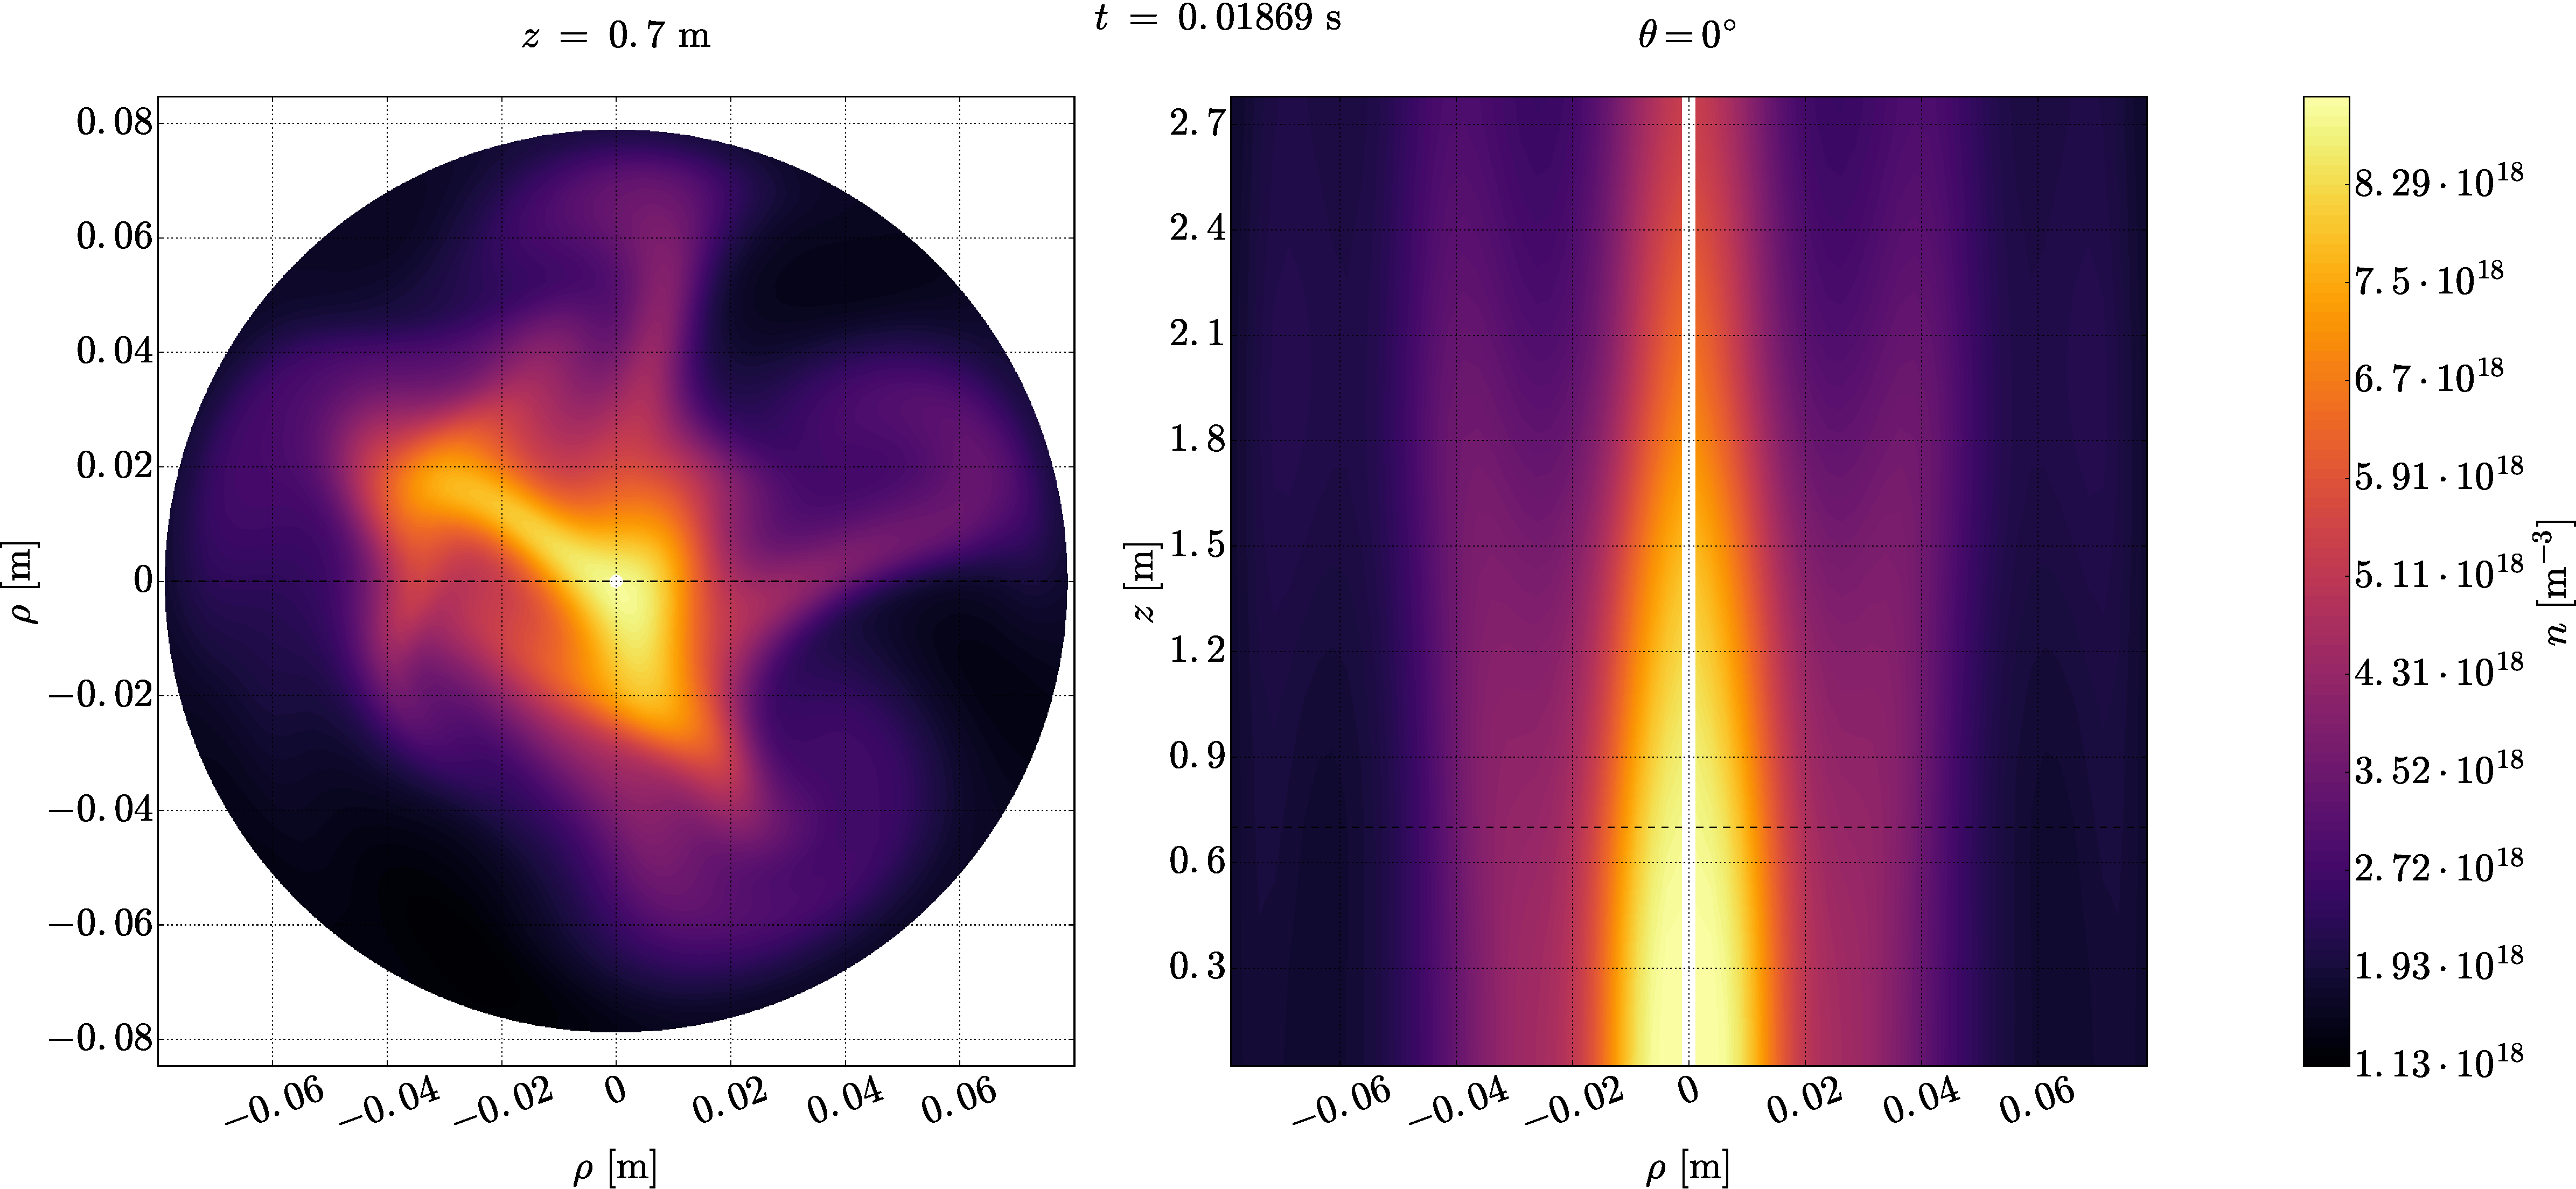
\includegraphics[width=1.0\textwidth]{fig/results/2DTurbulence/violentBurst}
        \caption{A violent burst is observed at the energy overshoot.}
        \label{fig:violentBurst}
    \end{subfigure}
    \\
    \begin{subfigure}[h]{1.00\textwidth}
        \centering
        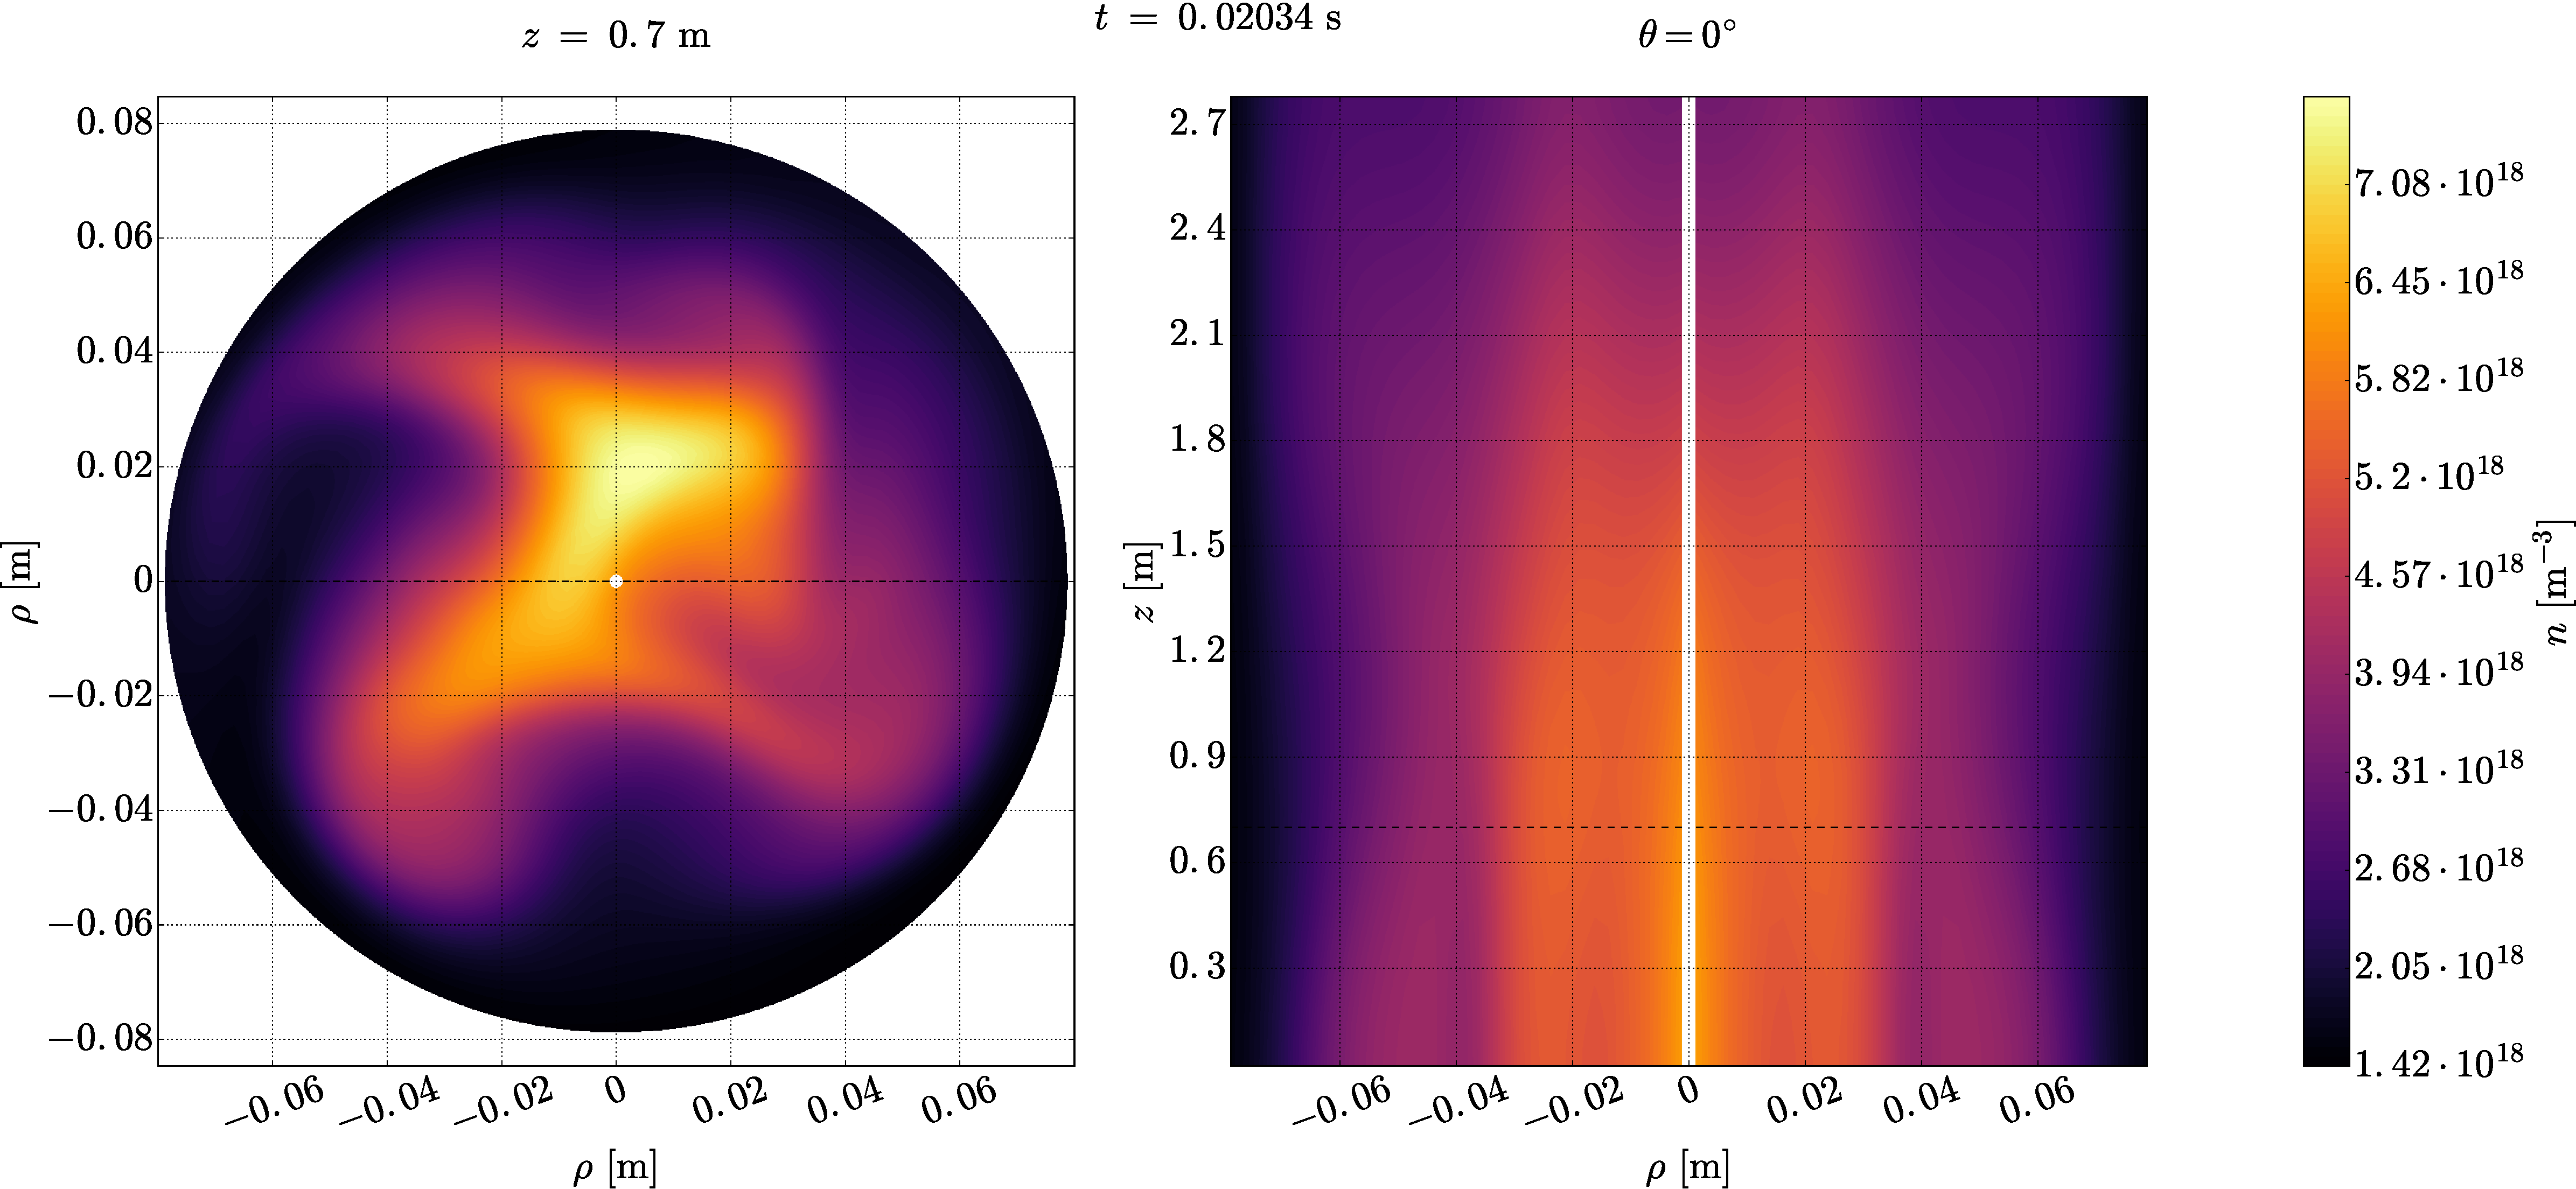
\includegraphics[width=1.0\textwidth]{fig/results/2DTurbulence/offCenter}
        \caption{Example of the plasma bulk being off axis}
        \label{fig:offcenter}
    \end{subfigure}
    \caption{Turbulent eddies are observed in the saturated turbulence state.
    Here shown for $B=0.1\T$}
\end{figure}
%
In the saturated turbulence state, the fluctuations are no longer in an ordered pattern as they were in the linear phase.
\Cref{fig:2DFluct} shows this.
%
\begin{figure}[htb]
    \centering
    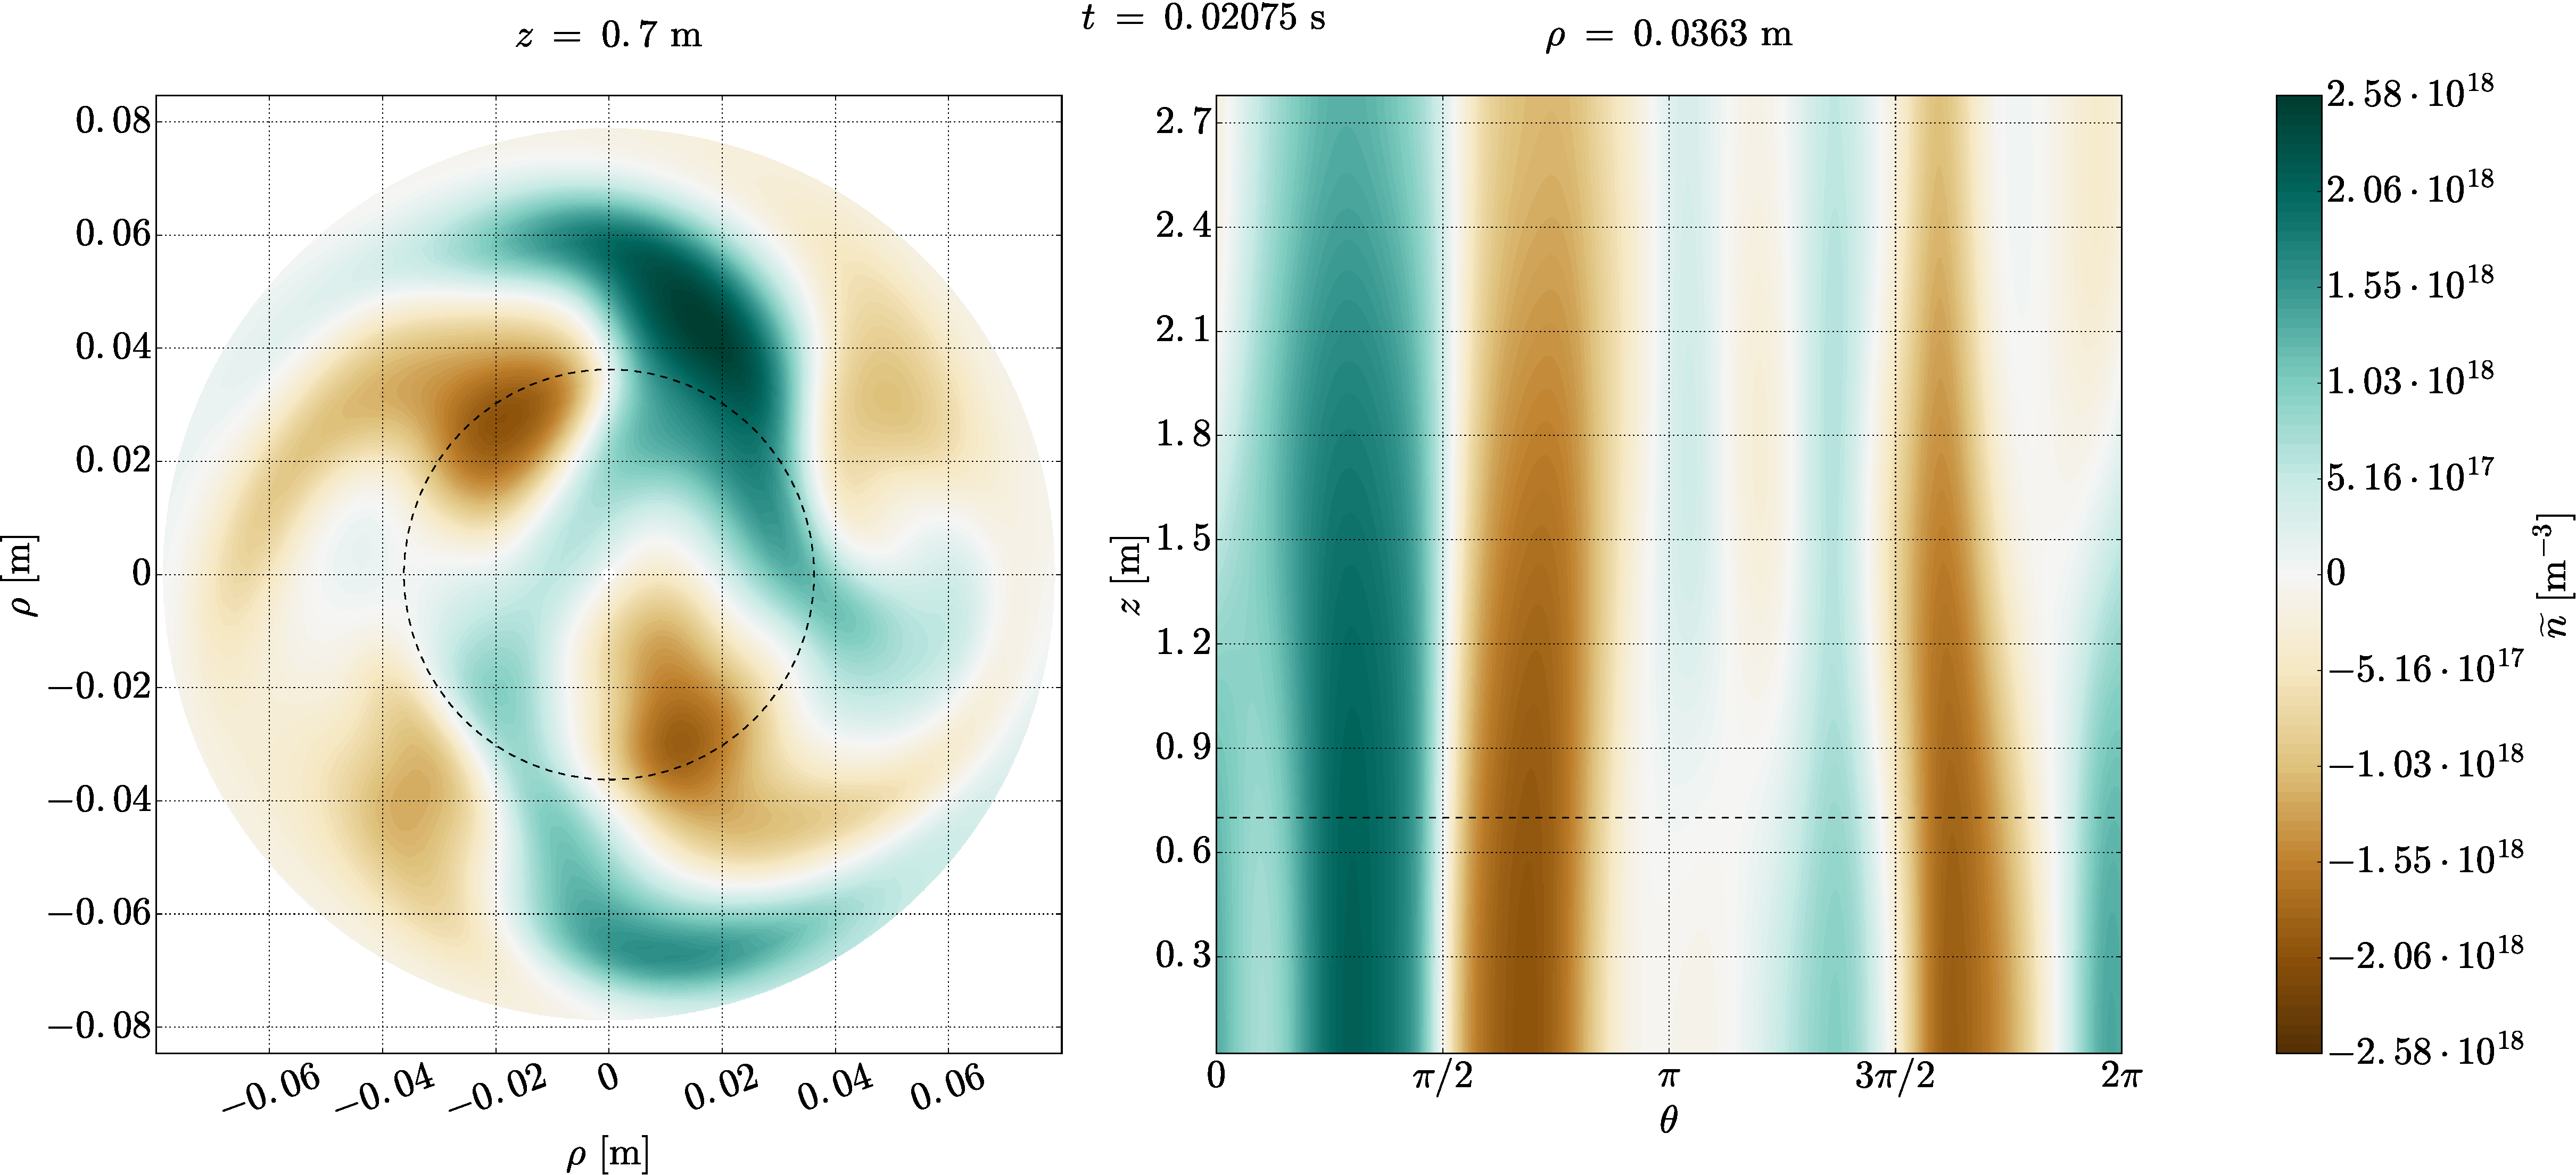
\includegraphics[width=1.0\textwidth]{fig/results/2DTurbulence/fluct}
    \caption{Fluctuations in the turbulent state for $B=0.1\T$}
    \label{fig:2DFluct}
\end{figure}
%
